\documentclass[a4paper]{article}
\usepackage{graphicx}
\usepackage{wrapfig}
\usepackage{float}
\usepackage[rightcaption]{sidecap}
\usepackage[top=1.25in, bottom=1.25in, left=1.25in, right=1.25in]{geometry}
\usepackage[style=authoryear, firstinits=true, backend=bibtex]{biblatex}
\usepackage{listings}
\usepackage{chngcntr}
\usepackage[titletoc,title]{appendix}
\addbibresource{references.bib}
\graphicspath{{images/}}
\usepackage{soul}
\usepackage{xcolor}
\usepackage[utf8]{inputenc}
\usepackage{pdfpages}
\usepackage{array}
\usepackage{acro}
\usepackage{makecell}
\usepackage{tabularx}
\usepackage{nicefrac}

\newcolumntype{L}[1]{>{\vspace{0pt}\raggedright\let\newline\\\arraybackslash\hspace{0pt}}m{#1}}
\newcolumntype{C}[1]{>{\vspace{0pt}\centering\let\newline\\\arraybackslash\hspace{0pt}}m{#1}}
\newcolumntype{R}[1]{>{\vspace{0pt}\raggedleft\let\newline\\\arraybackslash\hspace{0pt}}m{#1}}

% Add comma and space after Author name
\renewcommand*{\nameyeardelim}{\addcomma\addspace}

% Show roman numerals in section
% \renewcommand{\thesection}{\Roman{section}}

\definecolor{mygreen}{rgb}{0,0.6,0}
\definecolor{mygray}{rgb}{0.5,0.5,0.5}
\definecolor{mymauve}{rgb}{0.58,0,0.82}

% Set Language
\lstset{
	% list of keywords
	morekeywords={
		ns,
		declare,
		def,
		defn,
		println,
		doseq,
		cond,
		case,
		if,
		:else,
		else,
		throw,
		module,
		function
	},
	backgroundcolor=\color{white},
	basicstyle=\footnotesize,
	breakatwhitespace=false,
	breaklines=true,
	captionpos=b,
	commentstyle=\color{mygreen},
	deletekeywords={...},
	escapeinside={\%*}{*)},
	extendedchars=true,
	frame=single,
	keepspaces=true,
	keywordstyle=\color{blue},
	otherkeywords={*,...},
	numbers=left,
	numbersep=5pt,
	numberstyle=\tiny\color{mygray},
	rulecolor=\color{black},
	showspaces=false,
	showstringspaces=false,
	showtabs=false,
	stepnumber=1,
	stringstyle=\color{mymauve},
	tabsize=2
}

\DeclareAcronym{jvm}{
	short = JVM,
	long  = Java Virtual Machine,
	class = abbrev
}

\DeclareAcronym{tdd}{
	short = TDD,
	long = Test-Driven Development,
	class = abbrev
}

\DeclareAcronym{rad}{
	short = RAD,
	long = Rapid Application Development,
	class = abbrev
}

\DeclareAcronym{bnf}{
	short = BNF,
	long = Backus-Naur Form,
	class = abbrev
}

\DeclareAcronym{lifo}{
	short = LIFO,
	long = Last In First Out,
	class = abbrev
}

\begin{document}
	\pagenumbering{roman}
	\counterwithin{table}{section}
	\counterwithin{figure}{section}
	\counterwithin{lstlisting}{section}
	\title{Evaluation Report:\\Implementation of a compiler for Ralang}
	\author{Daniel Pacheco\\
		School of Computing and Digital Technology\\
		Faculty of Computing, Engineering and Built Environment\\
		Birmingham City University\\
		\texttt{Daniel.Pacheco@mail.bcu.ac.uk}}
	\date{\today}
	\maketitle
	\newpage
	\tableofcontents
	\newpage
	\listoftables
	\listoffigures
	\lstlistoflistings
	%\printacronyms[include-classes=abbrev,name=Abbreviations]
	\newpage
	\pagenumbering{arabic}
	\setcounter{page}{1}
	\vspace*{\fill}
	\begin{abstract}
		The purpose of this report is to evaluate the design and implementation of Ralang, an educational programming language designed to simplify and compliment the teaching of functional programming concepts to Computer Science undergraduates.\\
		
		The project lasted 12 consecutive weeks, involving research, design, implementation and testing, which included developing a product, a presentation and a viva of the overall project, a demonstration of the finished software and the final work: this report, which critically analysis and discusses the overall project.
	\end{abstract}
	\vspace*{\fill}
	\newpage
	\section{Introduction}
	\label{Sec:Intro}
	This evaluation report for the implementation of a compiler identifies and evaluates the successes and failures of the last 12 weeks of designing, developing and testing the product proposed in week 4. Part of the proposal is appended in appendix \ref{App:ProposalIntro} and appendix \ref{App:ProposalDesign}.\\
	
	Section \ref{Sec:Objectives} analyses project proposal, specifically the aims and objectives, then it attempts to identify if the initial system requirements were met within the amount of time available. This section will also be looking at the successes and failures of the project as a whole, nevertheless an in-depth analysis of  improvements and recommendations will only be discussed in section \ref{Sec:AnalysisAndDiscussion}.\\
	
	In the methodology, design and implementation section, we will briefly talk about some of the problems faced during the implementation and how the research replaced the designing stages and it affected the work flow of the project. The report covers some of the tools which were of use in the design and development stages: these tools were vital to the development and completion of Ralang.\\
	
	Section \ref{Sec:MDI} also mentions some of the most important problem we faced during the testing phase, nonetheless it's important to mention that some of these issues were found during the development process, others during the presentation and demonstration. An in-depth analysis of this was very important and will be discussed in section \ref{Sec:AnalysisAndDiscussion}.\\
	
	The testing section covers 2 very import types of testing used during the development of the project as well as a covering the evaluation of the results obtained from a questionnaire which were used to analyse the non-function requirements of Ralang. Most of the functional requirements will be analysed in section \ref{Sec:MDI} and \ref{Sec:AnalysisAndDiscussion} therefore it wasn't the focal point of this section.\\
	
	Until this point, the report has been preparing the material required to create a very critical and comprehensive analysis of the overview of the product and also the project. Section \ref{Sec:AnalysisAndDiscussion} proposes changes which will affect Ralang in the future. To create an in-depth discussion only a few important selected points will be discussed. In this section, the report will attempt to suggest ways of improving the methodologies, implementation or design, and also their approaches to each individual problem.\\
	
	Section \ref{Sec:AnalysisAndDiscussion}, may attempt to provide guidance to take on a similar project, or may attempt to suggest what other approaches might have been more suitable for a particular problem. Not only this but section \ref{Sec:AnalysisAndDiscussion} will be justifying reasons to why certain decisions had to be made, for instance why the testing methodology had to be adapted and why we were unable to use the proposed implementation methodology.\\
	
	Part of section \ref{Sec:AnalysisAndDiscussion}, will be reviewing the product and also the project management process. This will be based on the testing and evaluation, and will be concluding this section.\\
	
	Section \ref{Sec:Conclusion} will be looking at the highlights of this project by referring to the original aims, objectives and requirements which were added to appendix \ref{App:ProposalDesign}. We will use this section to create an overview of the project as a whole and also making recommendations for further research. Most importantly ensuring the objectives were met to the highest standard possible.
	\newpage
	\section{Achievement of Objectives}
	\label{Sec:Objectives}
	The software part of this project, to design and implement a programming language, has been mostly successful, as section \ref{Sec:Test} will be able to demonstrate in more detail that the 3 main objectives were met within the time frame specified by the project proposal. For more details about the aims and objectives in the proposal see appendix \ref{App:ProposalIntro}.\\
	
	A small group of students were asked to look at the source code of a program written in Ralang and were asked to answer a questionnaire to find out if the syntax of the language is readable and easy to follow. The results of this questionnaire, as depicted in figure \ref{fig:survey_results_1} shows that 3 out of 9 strongly agree that Ralang's syntax is readable and easy to follow, whilst 5 out of 9 agree that Ralang's syntax is readable and easy to follow, and 1 person does not have an opinion.\\
	
	\begin{figure}[h!]
		\centering
		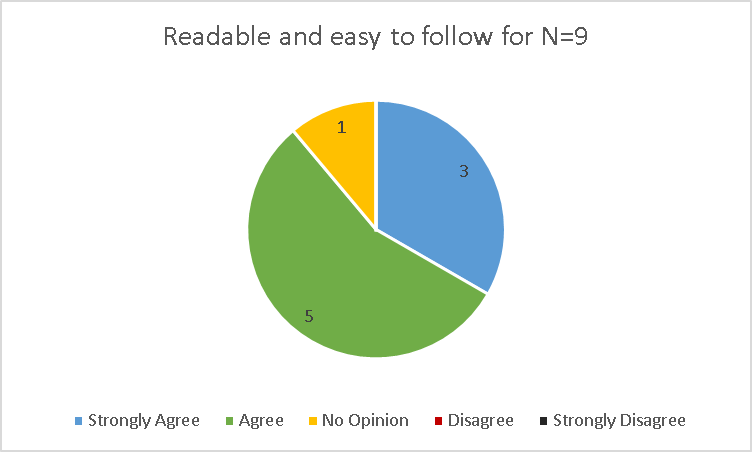
\includegraphics[width=0.9\linewidth]{images/survey_results_1.png}
		\caption[Survey results for Ralang appears to be readable and easy to follow]{Survey results for Ralang appears to be readable and easy to follow}
		\label{fig:survey_results_1}
	\end{figure}
	Ralang compiler is able to generate \ac{jvm} bytecode and run programs written in Ralang both on Windows 10 32-bit and Ubuntu 15.10 64-bit. Seventeen different test cases were used to test the compiler working on these 2 operating systems. For more details about compiling and running these test cases see appendix \ref{App:Running}. There are test cases which were identified to fail, these test cases will be studied in greater detail in section \ref{Sec:AnalysisAndDiscussion}, listed below are known reasons why some test cases are failing:
	\begin{itemize}
		\item \ac{lifo} Operand Stack limit set too low
		\item Local variables limit set too low
		\item \ac{jvm} level stack overflow
	\end{itemize}
	The tests mentioned above can be classified as system testing or black-box testing, where given a certain input then the output could be predicted and tested against. This type of testing was part of the methodology used in development, more details in section \ref{Sec:Test}.\\
	
	Unit tests were also developed to test specific functionality within the compiler which are known to break very easily for example the tokens obtained from the parser, when the \ac{bnf} file is changed. A total number of 72 different unit tests, to 1 of which is currently failing, as illustrated in figure \ref{fig:unit_test_results}.\\
	
	\begin{figure}[h!]
		\centering
		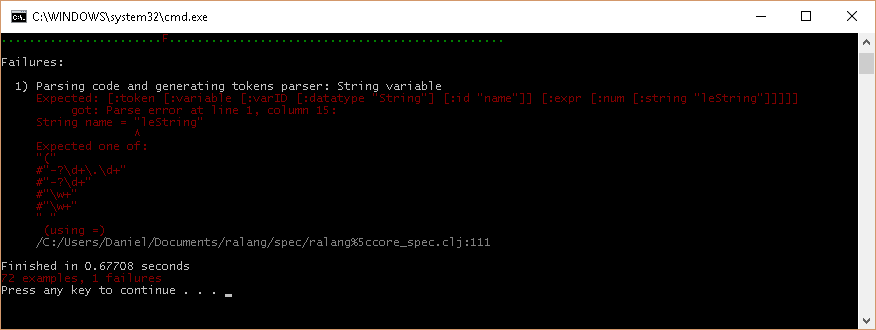
\includegraphics[width=\linewidth]{images/unit_test_results.png}
		\caption[Running 72 different unit test on Windows 10 32-bit]{Running 72 different unit test on a Windows machine}
		\label{fig:unit_test_results}
	\end{figure}
	The first 4 weeks of this project were used to plan and understand the feasibility of the project, by the fourth week a proposal was written formulating what system to target, as well as programming language choice to develop the compiler.\\
	
	Language design was planned to take place between week 4 and 6. Then the implementation of the compiler  would be between week 6 and 10. The last 2 weeks would be used to test the software and to ensure the language was consistent throughout. Due to lack of knowledge of compiler writing, the research had to take the place of design stage. Design of the language was worked out during the development stages instead.\\
	
	There was some aspects of the proposal which weren't well thought out, for example language design was poorly researched and it meant to finish the project by the twelfth week, a new approach to the problem had to take place. Overall, the 3 main objectives were met, nevertheless the development methodologies had to be adaptive.
	\newpage
	\section{Methodology, Design and Implementation}
	\label{Sec:MDI}
	As briefly discussed in appendix \ref{App:DevelopmentMethodology} about the proposed development methodologies, \ac{rad} software development methodology would be suitable for a project this size limited by the amount of time given if had it been researched and if appropriate designs for the language had been done prior to development. The project had to adapt a new methodology called \ac{tdd} in order to achieve the goals proposed. \\
	
	Figure \ref{fig:test_driven_development} shows the development stages of the compiler. Test cases are created to demonstrate and define the syntax of program's written in Ralang. One of the first test cases created was a hello world (testcases/helloworld.ra) which can be found in appendix \ref{App:Running}. In the test phase, it was also important to define what the outcome of that program after being executed should be. For instance, the hello world program was going to be able to display a message on the screen with the text "Hello World".\\
	
	\begin{figure}[h!]
		\centering
		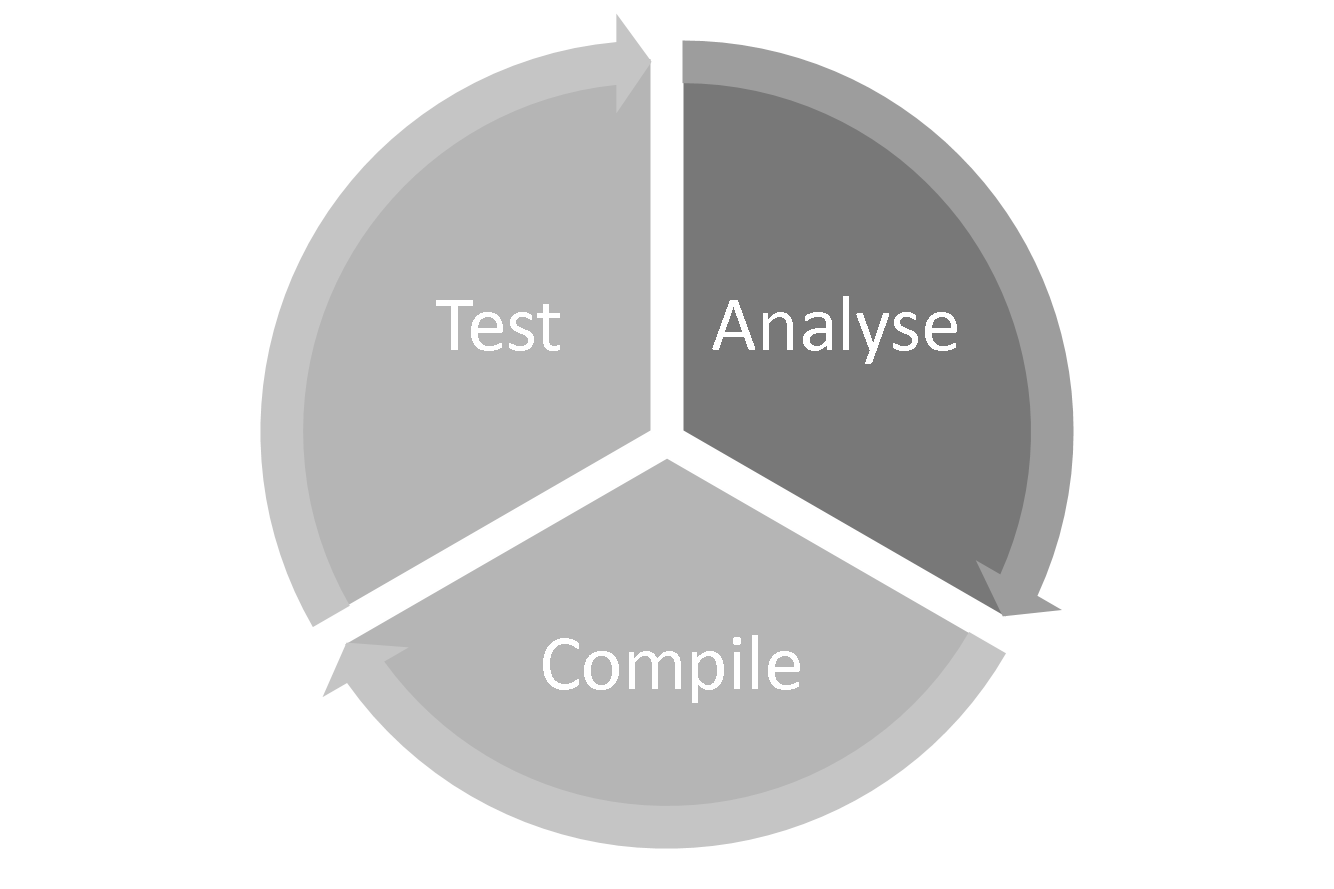
\includegraphics[width=0.7\linewidth]{images/test_driven_development.png}
		\caption{Test-driven development diagram showing development methodology}
		\label{fig:test_driven_development}
	\end{figure}
	The next 2 stages are more challenging because it requires understanding of the \ac{jvm} specification, the current state of the parser's grammar and to ensure the implementation is consistent throughout and that new test cases won't change the meaning of the language.\\
	
	Analyse stage consisted of looking for ways to interpret source code and trying to understand what the \ac{jvm} bytecode would have to look like in order to obtain the expected results from a particular test case. For that to work, different tools were used:
	\begin{itemize}
		\item Javap, is the Java class file disassembler. Sample Java programs could be compiled to a class file, and then \ac{jvm} bytecode could be studied.
		\item Jasmin, is an assembler for the \ac{jvm}, that allowed the creation of sample programs written in bytecode to be assembled into a class file to be executed.
		\item Bytecode Viewer, another Java class file disassembler with features to view Java code, to assist comparing the two high level languages, Java and Ralang.
	\end{itemize}
	Compiling stage involved generating bytecode from the sample test. This stage alone required several attempts until a workable version was produced. The testing part of development was only a small part of what the system required to be tested. Other testing methodologies had to be put in place to guarantee the system works as expected.\\
	
	A short survey was carried out in week 11, this helped to get feedback from people who have never seen this programming language before. There was not much time for planning and designing a comprehensive questionnaire but it allowed people to give quick feedback based on some sample code presented to them. A comprehensive qualitative and quantitative analysis of the results will be presented in greater details in section \ref{Sec:Test}. This questionnaire will be of use to further improve Ralang in the future.\\
	
	Testing was overall challenging, considering the fact that to meet the essential requirements of the project, the compiler had to be capable of working out the correct output for various inputs.\\
	
	Frequently during the development of this project, test cases which were able to compile properly previously, were unable to generate the correct bytecode after additions or changes in the system, and therefore the compiler would have to be fixed and all the prior test cases had to be tested against repeatedly throughout which slowed down the development of the project and that's when automated testing was introduced to tackle this issue.\\
	
	Unit tests were mostly focused around the parser, because those were the changes most problematic. For example if the grammar of the \ac{bnf} file had been changed to classify an Integer as a Number, and a Float was added to the grammar, but the Float was not added to be classified as a Number, the parser would  produce the wrong set of tokens but the error would only be detected during the code generation.\\
	
	Unit tests coverage are very extensive around the parser and the core of the compiler, nevertheless there is a lack of unit tests for the code generator. It would be useful to have more unit tests for the generator but for the purpose of this project it wouldn't be particularly important as Clojure would provide long stacktraces to allow the debugging of the software, as well as wrong generated bytecode could very easily be identified.\\
	
	\begin{figure}[h!]
		\centering
		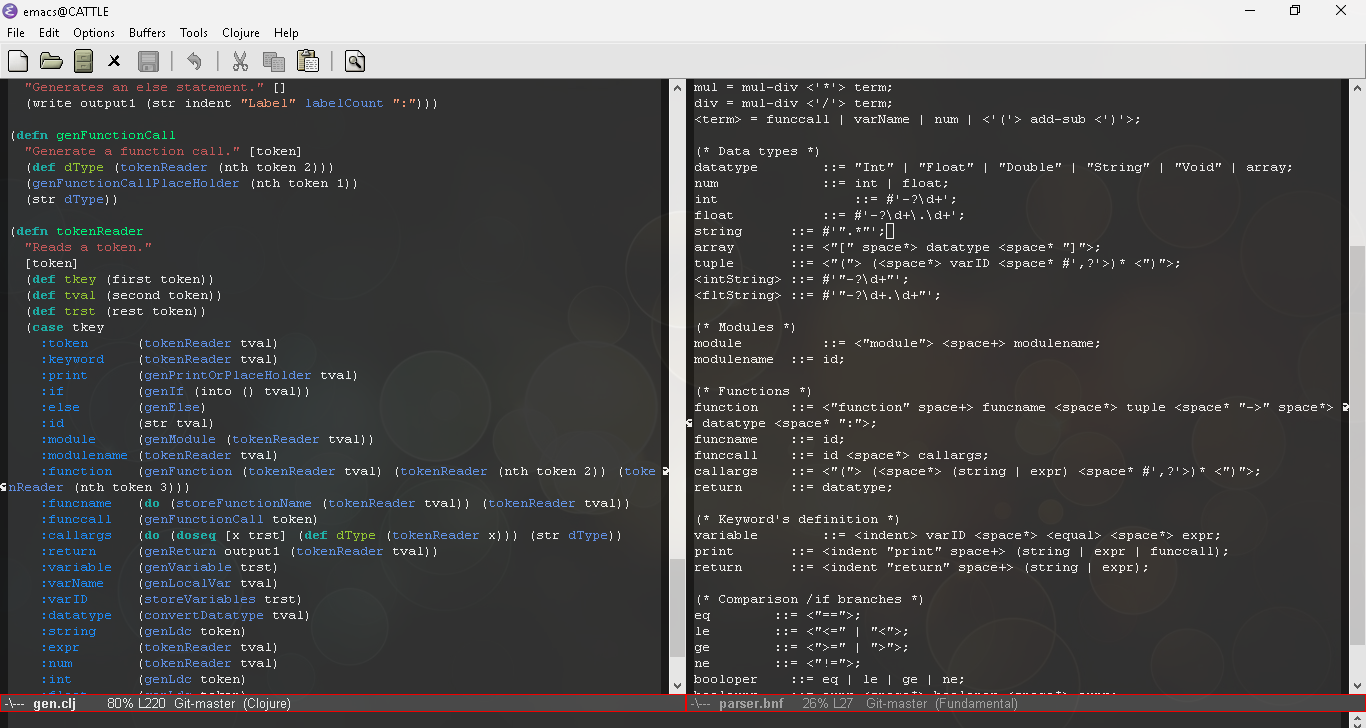
\includegraphics[width=\linewidth]{images/development_environment.png}
		\caption{Emacs used as a development environment for developing Ralang}
		\label{fig:development_environment}
	\end{figure}
	The project was developed on an Intel i3-2330M processor, with 4GB of RAM and on a 64-bit Windows 10 operating system, where certain Integrated Development Tools are unable to perform well such as Visual Studio and IntelliJ. Figure \ref{fig:development_environment}, shows Emacs text editor which allowed Ralang to be developed. It doesn't provide auto-completion or visual debuggers as expressed by \textcite{WhyEmacs}, but it works well with Clojure and performance wise is fast for the machine used to develop the system. Advanced techniques involved using keyboard shortcuts which increased performance immensely. \textcite{EmacsManual} was very useful for that purpose, and their software is very well documented.\\
	
	Clojure, as briefly mentioned in appendix  \ref{App:ProposalDesign}, was a good choice of programming language to be used in this project because it is a functional programming language which ensures functions do not have side effects, data structure manipulation is incredibly powerful in Clojure and it already runs on the \ac{jvm}, so for example, testing Ralang on a Linux machine works exactly the same way, after all the tools have been installed. Nevertheless learning a new language in such a small amount of time can be challenging, but there were many resources available online:
	\begin{itemize}
		\item StackOverflow.com had very helpful answers to questions which have been asked repeatedly over time. There was transferable knowledge from other programming languages, but it was more about learning how to do it the way Clojure compiler likes to interpret it. For instance, writing \textit{cond (conditions)} or \textit{case (switch cases)} were preferable to using \textit{if}.
		\item Clojure.org has got a detailed documentation with a lot of sample code. In the early stages of the development this was the place to learn the language, mainly Clojure's rich set of immutable data structures and extensive ways to manipulate these structures.
	\end{itemize}
	The two mostly used data structures were maps and lists. The parser returned a map of tokens as a binary tree, the generator would walk the tree and generate bytecode from the tokens. Variables, functions and their corresponding values, were stored in lists, and Clojure was able to provide a good toolkit to perform operations on these data structures.
	\newpage
	\section{Testing}
	\label{Sec:Test}
	The testing stage of the project was briefly discussed in the previous section, mainly the functional requirements. This section will attempt to give an overview of the functional requirements and explore in more detail the non-function requirements instead.
	\subsection{Functional requirements}
	In section \ref{Sec:MDI} it was discussed that testing was part of the development methodology, where a test case was created and then the implementation of the system resolved around that one scenario. After the system had been developed to work for that particular test case, testing every other scenario prior to that one was must, because making changes to the compiler may break some of the other parts which was previously working.\\
	
	This way of testing was not very time efficient, so unit tests were developed to check for changes in the parser which should remain the same, but in a more automatic and time efficient way. So when a change takes place, the unit tests are able to detect those changes and warn of certain problems the compiler may have.\\
	
	Section \ref{Sec:AnalysisAndDiscussion} will be evaluating and discussing these 2 different types of testing mentioned above and also the questionnaire results, in appendix \ref{App:Questionnaire}, in more detail.
	\subsection{Non-functional requirements}
	In this section, the report focuses on understanding the user needs rather than the requirements set in the proposal. Below maintainability, reliability and scalability will be analysed in greater detail how they are used to test these user requirements.
	\begin{itemize}
		\item \textbf{Maintainability}, is important when a project starts to grow, to allow further development to give users the changes they need and want in the system. For the maintainability of the compiler to improve, documentation would have to be also improved, as the users of this system would be relying on the latest information provided to them via the documentation.
		\item \textbf{Reliability}, ensures that after each change to the compiler, it remains to work the way that people already using it are accustomed to. This is very important in compiler writing, because if the syntax of the language keeps changing constantly, projects depending on the language would have to keep updating to follow the current standards of the language, in which case users would find a more stable programming language to run their services.
		\item \textbf{Scalability}, allows the product to grow. During the development of this project, we added the building blocks for this programming language, but left enough room for improvements: to create a strong and static data typing system, more functional than it currently is, code-generation optimisation and tail call recursion optimisations, would be prioritised.
	\end{itemize}
	There was only one other non-functional testing which involved asking a group of 9 people to look at the source code for a program written in Ralang code and to give their views. The results are shown in table \ref{Tab:QuestionnaireResults} in appendix \ref{App:Questionnaire} and are visually represented in figure \ref{fig:questionnaire_evaluation}.
	\newpage
	\begin{figure}[h!]
		\centering
		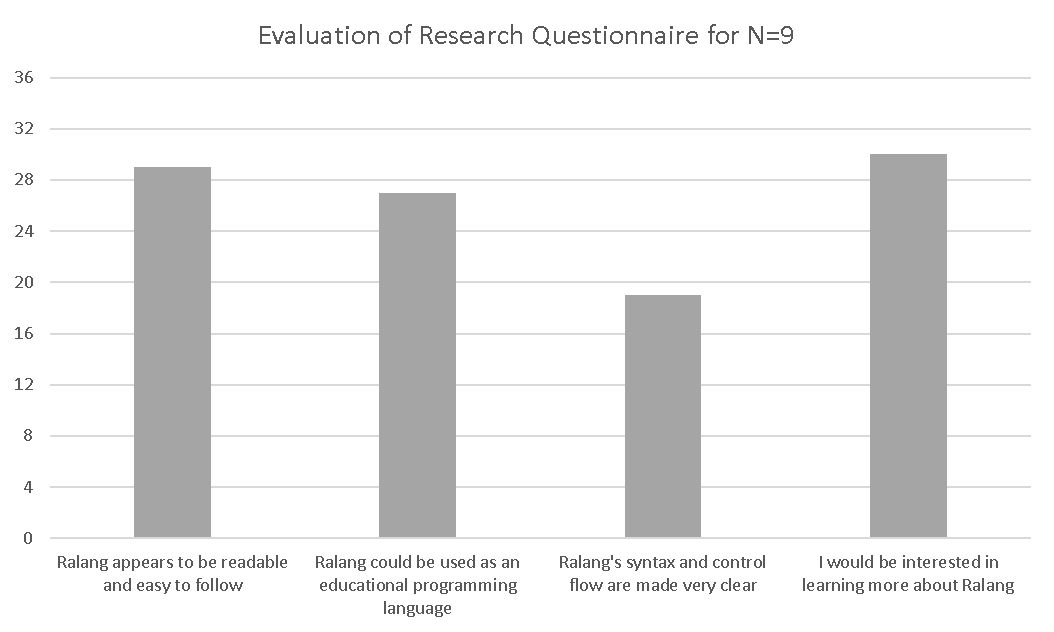
\includegraphics[width=0.8\linewidth]{images/evaluating_research_questionnaire.png}
		\caption{Evaluation of Research Questionnaire for a group of 9 students}
		\label{fig:questionnaire_evaluation}
	\end{figure}
	The results shown in figure \ref{fig:questionnaire_evaluation} are very optimistic, as over 80\% of the participants, have said the syntax of Ralang is readable and easy to follow and also that they would like to learn more about the programming language. Section \ref{Sec:AnalysisAndDiscussion} will be looking in more detail into the quality of this research.
	\newpage
	\section{Analysis, Discussion and Critical Appraisal}
	\label{Sec:AnalysisAndDiscussion}
	Until now the report has discussed what has been achieved in the last 12 weeks on this project, from the research and design stages, to the implementation and testing. The report covered the major problems encountered along the way but has not made any suggestions for improvements as of yet. In this section we will try to address anything that might have been overlooked, critically evaluating what has been done and suggesting alternatives to these issues.\\
	
	One of the problems which were briefly mentioned in section \ref{Sec:Objectives} and also during the product demonstration was the problems with stack and local variable limits being set too low and also \ac{jvm} level stack overflow. The reason for the stack and local variables limits being set too low is because each frame in the \ac{jvm} which has a \ac{lifo} operand stack and local variables, its maximum size need to be set at compile-time. \parencite{JVMSpec}
	\begin{figure}[h]
		\centering
		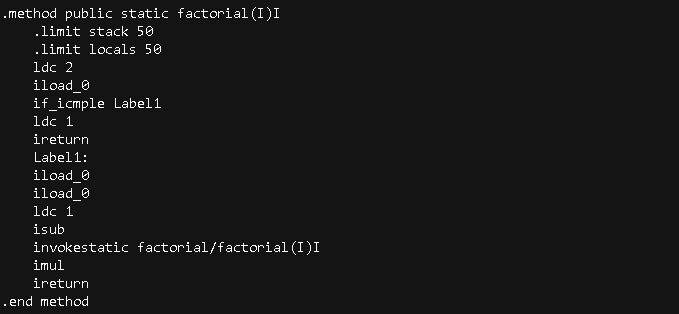
\includegraphics[width=\linewidth]{images/factorial_bytecode_sample.png}
		\caption{An example of a factorial function written in JVM bytecode}
		\label{fig:factorial_bytecode}
	\end{figure}\\
	During the implementation of the compiler, for quick prototyping, this operand stack and local variable limit was set to a static value of 50, as shown in figure \ref{fig:factorial_bytecode}, to give enough room to allow the test cases to run. Now this is a problem because if a program uses more space than it is allocated, it will still compile properly but the \ac{jvm} will not be able to run the program. There are a few approaches to tackle this problem:
	\begin{enumerate}
		\item \textbf{Creating a tag} in the place of \textit{.stack} and \textit{.local} (similar to the way function calls were dealt with), count the number of instructions, pushes, stores, etc. and then in the second-pass of the code-generation, updating these tags with their appropriate values.
		\item Generating \textbf{first-pass with default values of 0} being attributed to \textit{.stack} and \textit{.local}, calculating their true values during the second-pass of the code-generation and and lastly changing the default values to their correct values in a third-pass of the code-generation. With another pass, the compiler becomes slower because of the I/O stream speeds. It would be preferable to write/read as less as possible from the bytecode already generated.
		\item \textbf{Calculating the size required in the first-pass} by the \textit{.stack} and \textit{.local} before it gets written to the file. This is possible, if the data of each frame gets appended to a list, and after being able to calculate the size of the \textit{.stack} and \textit{.local}, only then the frame (method) gets written to the file all at once. This requires more memory to store the frame (from \textit{.method} to \textit{.endmethod}), and only then writing to the file.
	\end{enumerate}
	The first approach seems more reasonable than the other two. On one hand, the second option, requires too many reads and writes of the same file whilst the third option requires storing the whole method in memory and this could be critical in certain systems.\\
	
	The compiler already uses a two-pass code-generation, and the approach number 1 could take advantage of this. The size limit of \textit{.stack} and \textit{.local} would be calculated during the first-pass and would be written to the file in the second pass. This method would be saving memory in comparison with \textit{third} approach, and reducing the number of times writing to the same file in comparison with \textit{second} approach, increasing the overall performance of the compiler and its effectiveness.
	\begin{figure}[h!]
		\centering
		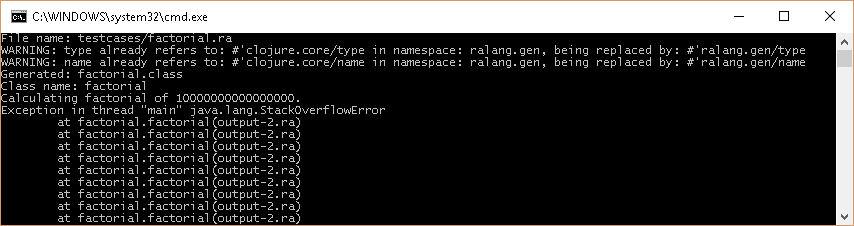
\includegraphics[width=\linewidth]{images/stack_overflow_sample.png}
		\caption{An example of a stack overflow}
		\label{fig:stack_overflow}
	\end{figure}\\
	The other problem which was identified during the demonstration was a StackOverflowError, as shown in figure \ref{fig:stack_overflow}. The \ac{jvm} throws a StackOverflowError if the computation in a thread requires a larger stack than the allowed amount, as described by \cite{JVMSpec}. There are a few approaches to tackle this problem:
	\begin{enumerate}
		\item Use \textbf{Clojure's approach} to the same problem by using \textit{java.lang.Long} to deal with integers and at the same time providing capabilities to use the \ac{jvm} primitive data types as shown in table \ref{Tab:JVMTypes}. Arguably though, if memory could be viewed as a critical in certain systems, using long to store a byte, short or int, may also cause some problems in the future. \parencite{TypedClojure}
		\item Use \textbf{\textit{java.lang.Integer} by default}, and automatically change the data type to a \textit{java.lang.Long} if the value is too large for an integer. This means the compiler will have to do extra checks and it also means we are moving away from a statically typed language, which would be one of the requirements for Ralang.
	\end{enumerate}
	For the time being, the first approach is easier to implement, nevertheless it would still be important to allow the creation of variables with different data types, in a similar way that Clojure does it. By doing so, the static typing is not being compromised and there is no need for extra checks in the compiler.
	\begin{table}[h!]
		\begin{tabular}{|l|c|c|}
			\hline Primitive data types & Start & End \\ 
			\hline Byte & -128 & 127 \\ 
			\hline Short & –32,768 & 32,767  \\ 
			\hline Int & –2,147,483,648 & 2,147,483,647 \\ 
			\hline Long & –9,223,372,036,854,775,808 & 9,223,372,036,854,775,807 \\ 
			\hline 
		\end{tabular}
		\caption{\ac{jvm} Numeric integral primitive data types excluding Char. Values obtained from \cite{JVMSpec}}
		\label{Tab:JVMTypes}
	\end{table}\\
	One last problem, which is important to mention and is not very obvious just by looking at figure \ref{fig:stack_overflow} and table \ref{Tab:JVMTypes} is that even though Ralang generates an integer by default changing it from a \textit{java.lang.Integer} to a \textit{java.lang.Long}, would not solve the stack overflow problem. It would still end up in a stack overflow error, as shown in figure \ref{fig:int_stack_overflow}.
	\newpage
	\begin{figure}[h!]
		\centering
		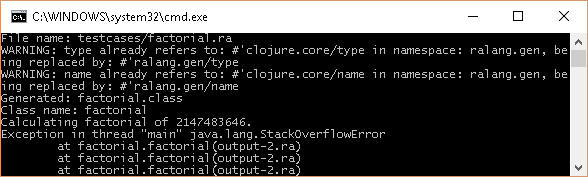
\includegraphics[width=\linewidth]{images/int_stack_overflow.png}
		\caption{An example of an Int resulting in a stack overflow}
		\label{fig:int_stack_overflow}
	\end{figure}
	The number (2147483646) used for this example is an integer still within the boundary limits of its type, nevertheless it is still causing a \textit{java.lang.StackOverflowError}. This happens because a recursive function which is not being optimised by the compiler, for instance a simple \textit{factorial(5)} calling factorial function in listing \ref{factorial} would generate similar results to the \textit{Without Optimisation} in table \ref{Tab:Optimisation}:
	\begin{table}[h!]
		\begin{tabular}[t]{|C{0.47\linewidth}|C{0.47\linewidth}|}
			\hline Without optimisation & With optimisation \\ 
			\hline \makecell[l]{factorial(5)\\
				=5 * factorial(4)\\
				=5 * 4 * factorial(3)\\
				=5 * 4 * 3 * factorial(2)\\
				=5 * 4 * 3 * 2 * factorial(1)\\
				=5 * 4 * 3 * 2 * 1\\
				=5 * 4 * 3 * 2\\
				=5 * 4 * 6\\
				=5 * 24\\
				=120} & \makecell[l]{factorial(5)\\
				=call\_factorial(5, 1)\\
				=call\_factorial(4, 3)\\
				=call\_factorial(3, 6)\\
				=call\_factorial(2, 24)\\
				=call\_factorial(1, 120)\\
				=120} \\
			\hline 
		\end{tabular}
		\caption{Comparing with and without optimisation code.}
		\label{Tab:Optimisation}
	\end{table}\\
	So not only, the approaches mentioned above would have to be implemented, but also tail call recursion optimisation, to prevent recursive calls from generating large chains of recursive calls. Now the problem with the number (2147483646) will generate such a long tail it will blow the stack. Since the \ac{jvm} does not implement tail call recursion, this would have to be implemented at the compiler level, a representation of this is shown in \textit{With optimisation} in table \ref{Tab:Optimisation} as described by \cite{JVMlanguages}, which was one of the suggestions for the Clojure compiler too.\\
	
	\cite{RecurInClojure} also warns that various modern programming languages don't implement because of the legacy tools and software, others because they were short-term thinking and others simply because there is not enough pressure to implement tail call optimisations. For Ralang, this was a design problem for not wanting to use looping techniques such as \textit{for} and \textit{while} loops, on the other hand it means that implementing appropriate recursive calls optimisations are essential for Ralang.\\
	
	The reason why Ralang has decided to stick to recursive calls only instead of \textit{for} and \textit{while} loops which are very common in modern programming languages, is because iteration over recursive calls would require the language to be in a mutable state, in which case it would be moving away from a purely functional programming language as intended for this project.\\
	
	In section \ref{Sec:MDI} and \ref{Sec:Test} it was covered 2 main types of testing and also a questionnaire which can be found in appendix \ref{App:Questionnaire}. It is important to mention that the design of the questionnaire is not thoroughly thought out and it was planned to remove as much ambiguity as possible, nevertheless it is important to keep in mind that all participants were people from the same faculty and it may still contain ambiguous responses. Hence why it is important to not rely too much on this particular questionnaire but instead to discuss how we might have been able to improve it for a different study:
	\begin{enumerate}
		\item Allow people to try out the software for themselves for a short period of time, this may require some form of tutorial to begin with, and then to allow them answering a questionnaire of the same sort. This will give the correspondents enough time and experience with the language before they are asked for their opinion.
		\item The questionnaire presented to these students, had a sample code in Ralang and also in C\#. As C\# was used at our university some students might have already created some sort of preconception about C\#, and this might have affected the results. This links back to point no. 1, if the students were allowed to try the software before they answered the questionnaire, this might have affected the results.
		\item Instead of a questionnaire, a simple test could be put in place, to see if the students actually learned how the programming language works, and based on these results then we could take the students feedback on board.
	\end{enumerate}
	These could be some potential solutions if a new research was to take place. Nevertheless, even though the other 2 tests were much more accurate, there still was a lot of room for improvements, mainly with the unit testing, but also with the \ac{tdd}, as can be shown in appendix \ref{App:Running}.\\
	
	The system tests, were missing a lot of important features and it did not test for system failures. This is really important, because during the demonstration and viva of the project several problems were discussed which were not identified during the system testing. It's arguable that during the development phase, these system tests were used to develop the product and not exactly to test every possible case scenario, and that is the reason why test cases were developed in the first place.\\
	
	Though, not even the unit tests can provide the most accurate results. The reason for this is because the coverage of the unit tests are very tiny for a project of this size. The unit tests coverage is about \nicefrac{1}{5} of the entire project. It does cover one of the most important parts which is the parser, which was one of the most difficult parts of the compiler to debug, nevertheless there is still a lot of ground to cover. The main reason why this was not completed was because there simply was not enough time.\\
	
	In terms of achieving the main objectives, three of the most important challenges faced, was researching compiler writing, the time frame allocated to the project and being able to quickly adapt to a new implementation methodology. As mentioned previously in section \ref{Sec:MDI}, replacing the design process with the research of compiler design, meant that there was not enough time to plan Ralang's language, therefore the approach taken was to design test cases and make the compiler to work for those particular test cases.\\
	
	The language slowly started to become very inconsistent throughout, and it meant re-thinking and re-implementing several parts. As a future reference, it would be very important to have the language design done first and peer-reviewed for inconsistencies and then implemented into the compiler, this would have saved half of the time, and the time lost could have been used improving the test cases, unit tests and looking into improving features in the language.\\
	
	Non-functional requirements in section \ref{Sec:Test} is a very important part of this project but it's one of the most difficult ones to test. This essentially is supposedly testing the user requirements for the language, and at this point is very difficult to carry out such type of testing. One of the point which was not mentioned in section \ref{Sec:Test} was that carrying out the following types of non-functional requirements would be very important:
	\begin{itemize}
		\item \textbf{Platform compatibility} would mean testing the compiler in other Operating Systems, like other versions of Windows and Linux, as well as Mac OS, possibly also targeting the Android platform.
		\item \textbf{Documentation}, to provide the users with access to an in-depth documentation, guides, and how-to, sample code, etc. This is very important to allow the users to feel empowered, when they are stuck to enable them to find the information as quickly as possible.
		\item \textbf{Performance and response time}, as in how fast does it take to perform a large task. This would require testing the system under a lot of stress and seeing how it performs, in a way or another, it could be considered also a stress test.
	\end{itemize}
	One last non-functional requirement that should have been tested more thoroughly was the \textbf{extensibility and reusability} test. As shown in appendix \ref{App:JavaIntegration}, the Java integration is something that would be very useful to integrate Ralang applications with Java applications. It would also be very useful to have it the other way around, and to allow the extensive Java Class Library to be imported into Ralang.\\
	
	It was a great accomplishment to enable the Ralang compiler to create a \textit{package} which then a Java program could import and make use of, as demonstrated in appendix \ref{App:JavaIntegration}. The next step would be to allow the Ralang compiler to import classes from Java Class Library, but this would require focusing on the language's current issues before adding additional features.
	\newpage
	\section{Conclusion}
	\label{Sec:Conclusion}
	The project design, implementation and testing followed the proposal (appendix \ref{App:ProposalIntro} and \ref{App:ProposalDesign}) in almost every aspect it could. The time frame was a bit off because of the research which had to be done in order to begin the design and implementation.\\
	
	The questionnaire involved handing out printed questionnaires and talking to people directly about the project. It was intended for the participants to get a tutorial and then attempt to program in Ralang, before answering the questionnaire. Due to the amount of time this was not possible, but may be considered in the future.\\
	
	It would be possible to use online surveys to get a lot more feedback, nevertheless for this project it was necessary to have a face-to-face conversation with people to make sure they understand what this project is all about and also to answer any questions. This process obviously is more time consuming but the results seem to be more genuine since the people who took part, seemed very engaged and wanting to know more about Ralang and also the project overall.\\
	
	Similarly, the development methodologies had to be changed in order to finish the product within the time frame. This was specially important because the proposal did not take the time it would take to research the implementation, and it took too long. Using the \ac{tdd} instead of the \ac{rad}, was not a terrible change, though in the future it may even be considered as a first option.\\
	
	With the testing, we went beyond what was in the initial specification and developed additional unit tests to provide a more efficient way of testing and guaranteeing the software works each time after any changes. Unit tests helped greatly in developing the system, as prior to week 9 all the manual tests were becoming harder to maintain. It greatly contributed towards providing quick feedback loops and enough debugging information when anything stopped working.\\
	
	The project management process, focused on getting the most basic test cases scenario to work first. The first test case scenario was one of the hardest because the \ac{jvm} was a new system which had to be learnt, as well as Clojure, the programming language of choice to write the compiler, had to be learnt from the ground up also, and writing a compiler was no easy task mainly to learn it and develop one at the same time. There was a basic idea of how it all was going to work together to read a source file and compile it into a \ac{jvm} class file, it is now represented in appendix \ref{App:HighLevelDesign}, and it is essentially the high-level design.\\
	
	This design was to keep in mind that a few compiler writing techniques were to be skipped in order to have enough time to create a basic one that works well. For instance, the parser was created using InstaParse for Clojure and the code optimisations would be a step which ought to be skipped to keep the project within the time frame.\\
	
	In the future, it would be great to work on optimised and specialised parser for Ralang and to have an optimised compiler which could generate optimised code for the \ac{jvm}, and perform compile-time function execution.
	\newpage
	\printbibliography
	\newpage
	\appendixpage
	\label{App:Appendices}
	\begin{appendices}
	\section{Source code for Ralang}
	\label{App:SourceCode}
	\subsection{src/ralang/core.clj}
	\lstinputlisting[caption="Source code for the main file of Ralang compiler"]{core.clj}
	\subsection{src/ralang/gen.clj}
	\lstinputlisting[caption="Source code for Ralang's token generator"]{gen.clj}
	\subsection{spec/ralang/core\_spec.clj}
	\lstinputlisting[caption="Source code for Ralang's unit tests"]{core_spec.clj}
	\subsection{resources/parser.bnf}
	\lstinputlisting[caption="Ralang's compiler \ac{bnf} context-free grammar"]{parser.bnf}
	\pagebreak
	\section{Running test cases}
	\label{App:Running}
	\subsection{Sample program's Source Code}
	\subsection{resources/parser.bnf}
	\lstinputlisting[caption="Program written in Ralang: testcases/callhello.ra"]{testcases/callhello.ra}
	\lstinputlisting[caption="Program written in Ralang: testcases/compare.ra"]{testcases/compare.ra}
	\lstinputlisting[caption="Program written in Ralang: testcases/complex.ra"]{testcases/complex.ra}
	\lstinputlisting[label=factorial, caption="Program written in Ralang: testcases/factorial.ra"]{testcases/factorial.ra}
	\lstinputlisting[caption="Program written in Ralang: testcases/funccall.ra"]{testcases/funccall.ra}
	\lstinputlisting[caption="Program written in Ralang: testcases/helloworld.ra"]{testcases/helloworld.ra}
	\lstinputlisting[caption="Program written in Ralang: testcases/legal.ra"]{testcases/legal.ra}
	\lstinputlisting[caption="Program written in Ralang: testcases/mulcomp.ra"]{testcases/mulcomp.ra}
	\lstinputlisting[caption="Program written in Ralang: testcases/mulfuncs.ra"]{testcases/mulfuncs.ra}
	\newpage
	\lstinputlisting[caption="Program written in Ralang: testcases/mulhello.ra"]{testcases/mulhello.ra}
	\lstinputlisting[caption="Program written in Ralang: testcases/multimaths.ra"]{testcases/multimaths.ra}
	\lstinputlisting[caption="Program written in Ralang: testcases/mulvars.ra"]{testcases/mulvars.ra}
	\lstinputlisting[caption="Program written in Ralang: testcases/notcompare.ra"]{testcases/notcompare.ra}
	\lstinputlisting[caption="Program written in Ralang: testcases/printnum.ra"]{testcases/printnum.ra}
	\lstinputlisting[caption="Program written in Ralang: testcases/subtwo.ra"]{testcases/subtwo.ra}
	\lstinputlisting[caption="Program written in Ralang: testcases/vars.ra"]{testcases/vars.ra}
	\lstinputlisting[caption="Program written in Ralang: testcases/varstring.ra"]{testcases/varstring.ra}
	\subsection{Linux - Ubuntu 15.10 64-bit}
	\begin{figure}[h!]
		\centering
		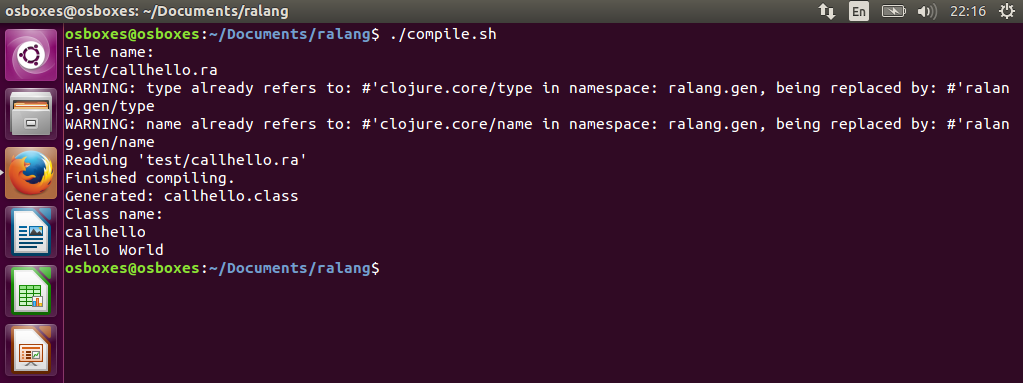
\includegraphics[width=\linewidth]{images/ubuntu_callhello.png}
		\caption[Compiling and running callhello.ra on Ubuntu 15.10 64-bit]{Compiling and running callhello.ra on Ubuntu}
		\label{fig:ubuntu_callhello}
	\end{figure}
	\begin{figure}[h!]
		\centering
		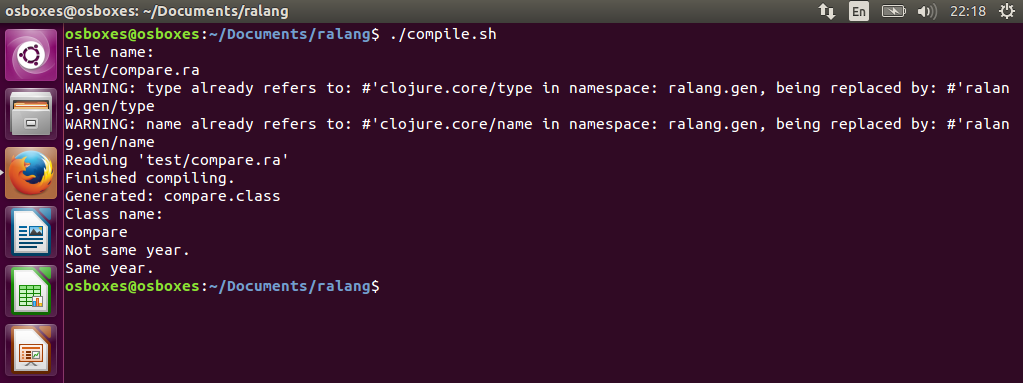
\includegraphics[width=\linewidth]{images/ubuntu_compare.png}
		\caption[Compiling and running compare.ra on Ubuntu 15.10 64-bit]{Compiling and running compare.ra on Ubuntu}
		\label{fig:ubuntu_compare}
	\end{figure}
	\begin{figure}[h!]
		\centering
		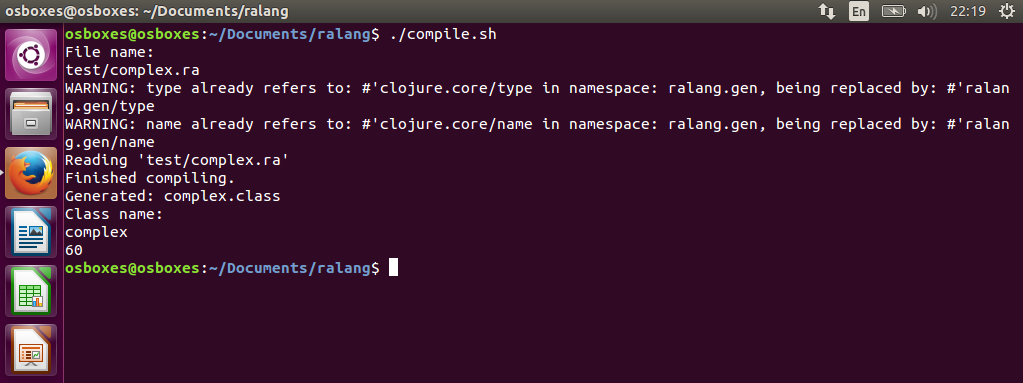
\includegraphics[width=\linewidth]{images/ubuntu_complex.png}
		\caption[Compiling and running complex.ra on Ubuntu 15.10 64-bit]{Compiling and running complex.ra on Ubuntu}
		\label{fig:ubuntu_complex}
	\end{figure}
	\newpage
	\begin{figure}[h!]
		\centering
		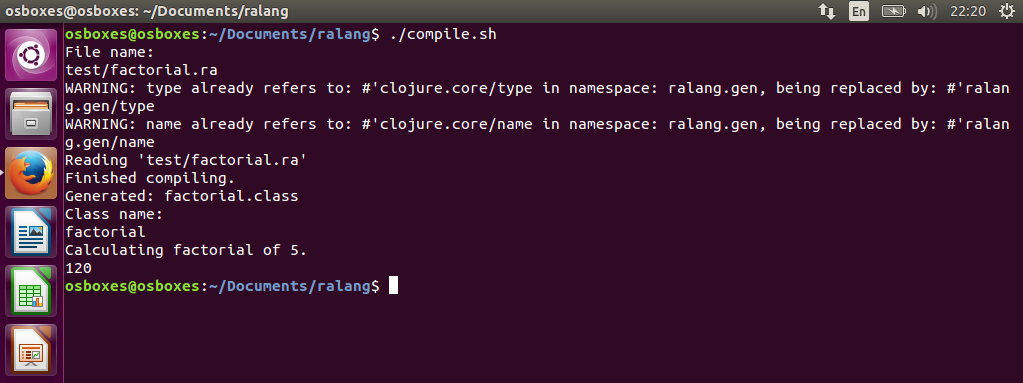
\includegraphics[width=\linewidth]{images/ubuntu_factorial.png}
		\caption[Compiling and running factorial.ra on Ubuntu 15.10 64-bit]{Compiling and running factorial.ra on Ubuntu}
		\label{fig:ubuntu_factorial}
	\end{figure}
	\begin{figure}[h!]
		\centering
		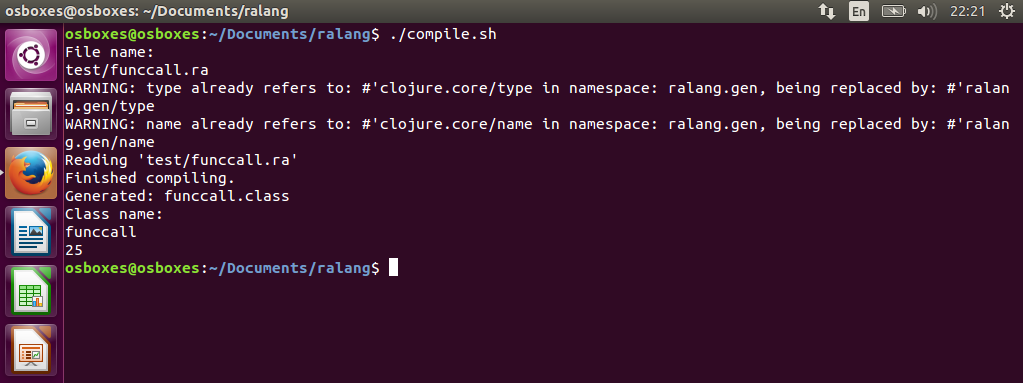
\includegraphics[width=\linewidth]{images/ubuntu_funccall.png}
		\caption[Compiling and running funccall.ra on Ubuntu 15.10 64-bit]{Compiling and running funccall.ra on Ubuntu}
		\label{fig:ubuntu_funccall}
	\end{figure}
	\begin{figure}[h!]
		\centering
		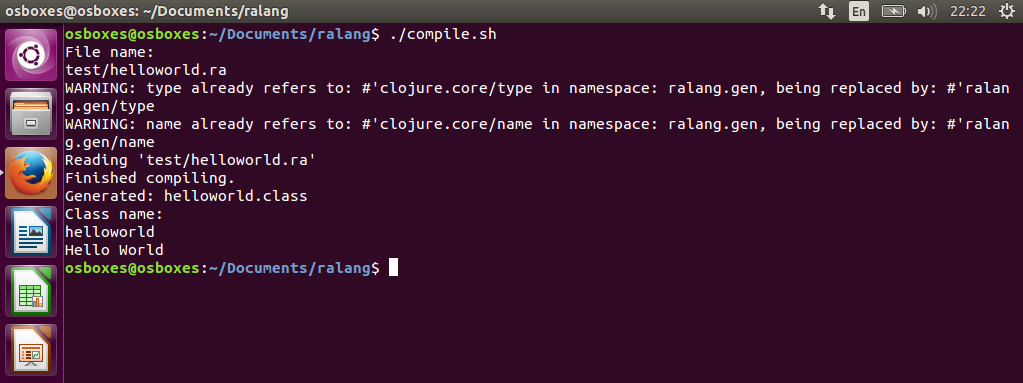
\includegraphics[width=\linewidth]{images/ubuntu_helloworld.png}
		\caption[Compiling and running helloworld.ra on Ubuntu 15.10 64-bit]{Compiling and running helloworld.ra on Ubuntu}
		\label{fig:ubuntu_helloworld}
	\end{figure}
	\newpage
	\begin{figure}[h!]
		\centering
		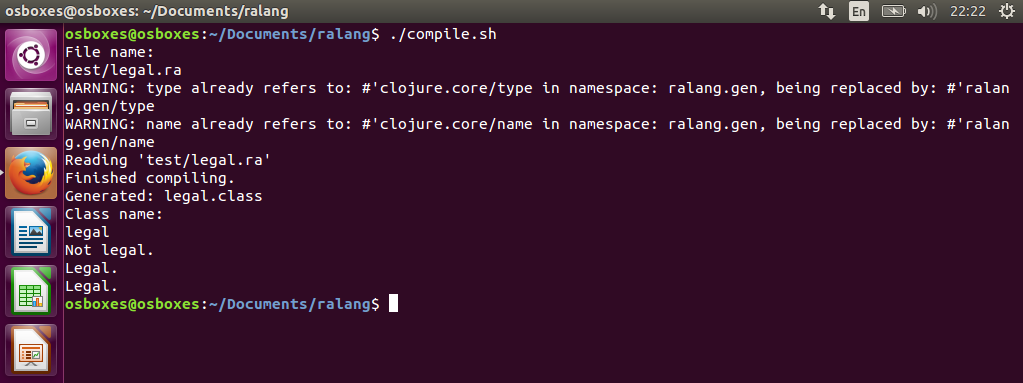
\includegraphics[width=\linewidth]{images/ubuntu_legal.png}
		\caption[Compiling and running legal.ra on Ubuntu 15.10 64-bit]{Compiling and running legal.ra on Ubuntu}
		\label{fig:ubuntu_legal}
	\end{figure}
	\begin{figure}[h!]
		\centering
		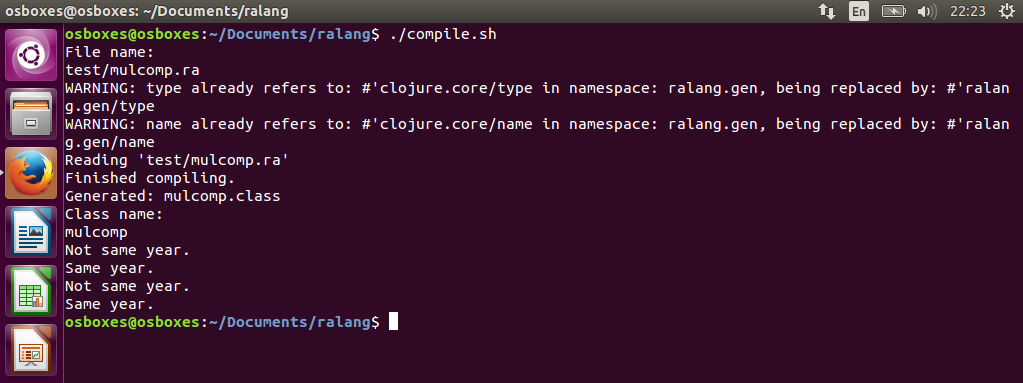
\includegraphics[width=\linewidth]{images/ubuntu_mulcomp.png}
		\caption[Compiling and running mulcomp.ra on Ubuntu 15.10 64-bit]{Compiling and running mulcomp.ra on Ubuntu}
		\label{fig:ubuntu_mulcomp}
	\end{figure}
	\begin{figure}[h!]
		\centering
		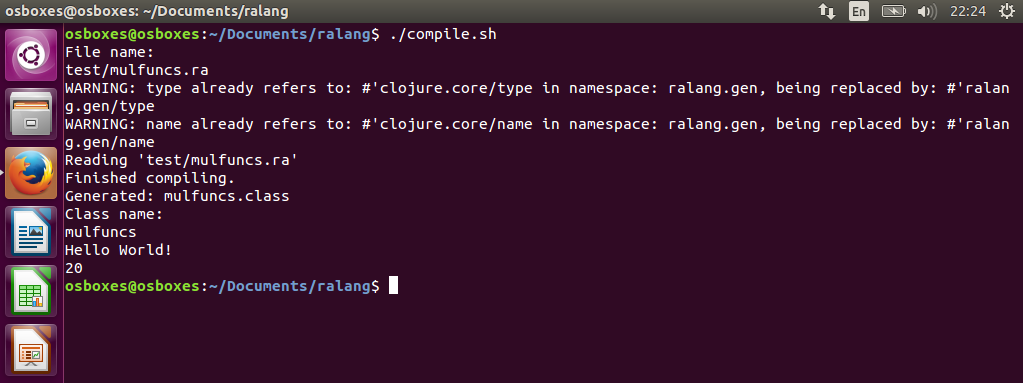
\includegraphics[width=\linewidth]{images/ubuntu_mulfuncs.png}
		\caption[Compiling and running mulfuncs.ra on Ubuntu 15.10 64-bit]{Compiling and running mulfuncs.ra on Ubuntu}
		\label{fig:ubuntu_mulfuncs}
	\end{figure}
	\newpage
	\begin{figure}[h!]
		\centering
		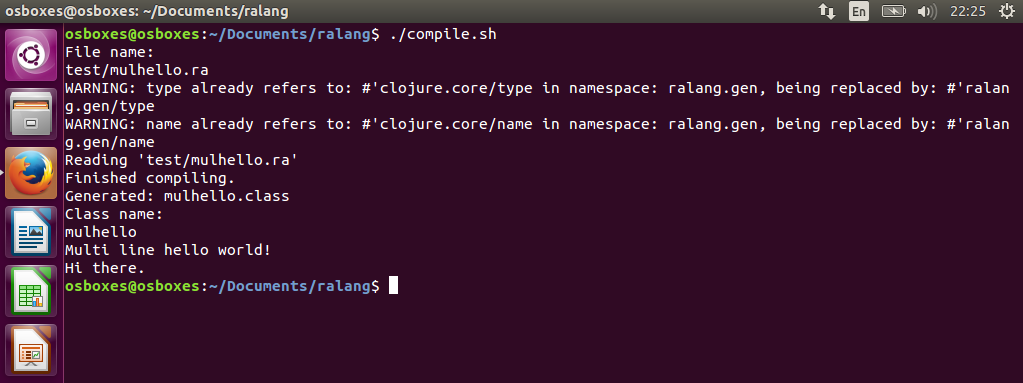
\includegraphics[width=\linewidth]{images/ubuntu_mulhello.png}
		\caption[Compiling and running mulhello.ra on Ubuntu 15.10 64-bit]{Compiling and running mulhello.ra on Ubuntu}
		\label{fig:ubuntu_mulhello}
	\end{figure}
	\begin{figure}[h!]
		\centering
		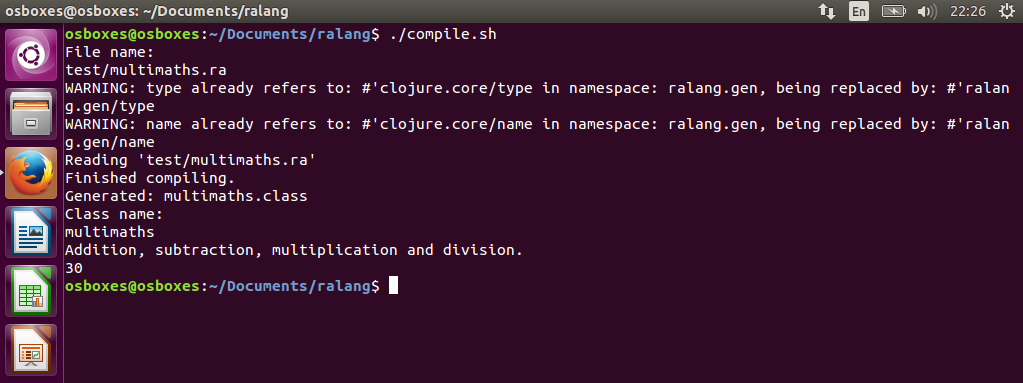
\includegraphics[width=\linewidth]{images/ubuntu_multimaths.png}
		\caption[Compiling and running multimaths.ra on Ubuntu 15.10 64-bit]{Compiling and running multimaths.ra on Ubuntu}
		\label{fig:ubuntu_multimaths}
	\end{figure}
	\begin{figure}[h!]
		\centering
		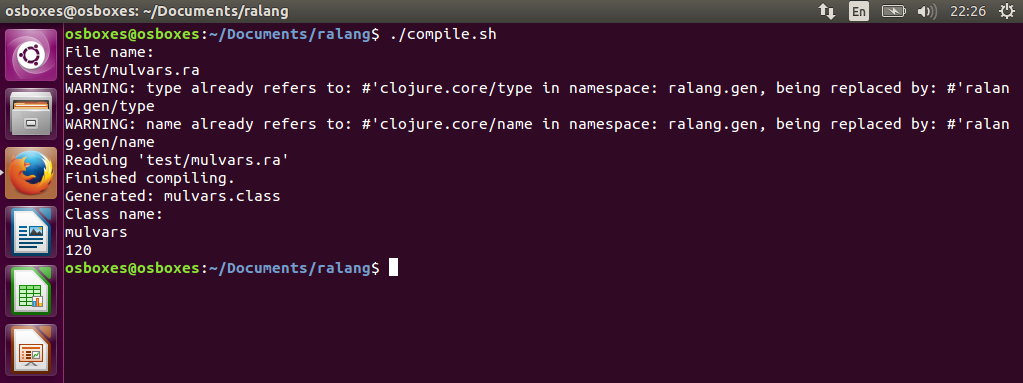
\includegraphics[width=\linewidth]{images/ubuntu_mulvars.png}
		\caption[Compiling and running mulvars.ra on Ubuntu 15.10 64-bit]{Compiling and running mulvars.ra on Ubuntu}
		\label{fig:ubuntu_mulvars}
	\end{figure}
	\newpage
	\begin{figure}[h!]
		\centering
		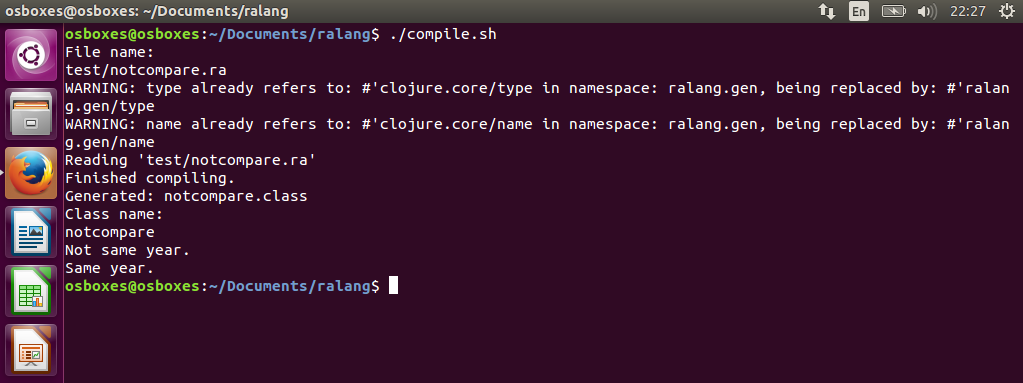
\includegraphics[width=\linewidth]{images/ubuntu_notcompare.png}
		\caption[Compiling and running notcompare.ra on Ubuntu 15.10 64-bit]{Compiling and running notcompare.ra on Ubuntu}
		\label{fig:ubuntu_notcompare}
	\end{figure}
	\begin{figure}[h!]
		\centering
		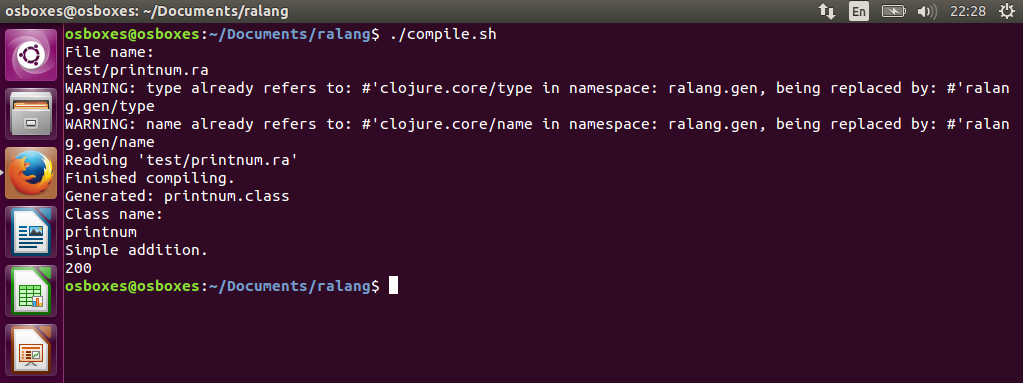
\includegraphics[width=\linewidth]{images/ubuntu_printnum.png}
		\caption[Compiling and running printnum.ra on Ubuntu 15.10 64-bit]{Compiling and running printnum.ra on Ubuntu}
		\label{fig:ubuntu_printnum}
	\end{figure}
	\begin{figure}[h!]
		\centering
		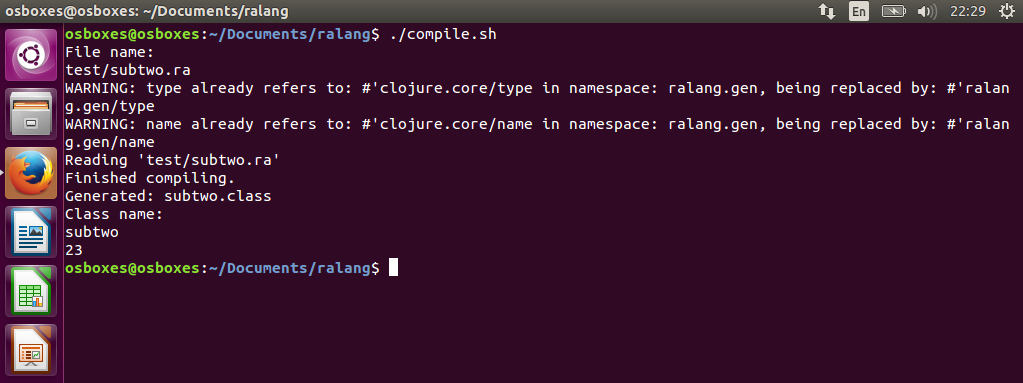
\includegraphics[width=\linewidth]{images/ubuntu_subtwo.png}
		\caption[Compiling and running subtwo.ra on Ubuntu 15.10 64-bit]{Compiling and running subtwo.ra on Ubuntu}
		\label{fig:ubuntu_subtwo}
	\end{figure}
	\newpage
	\begin{figure}[h!]
		\centering
		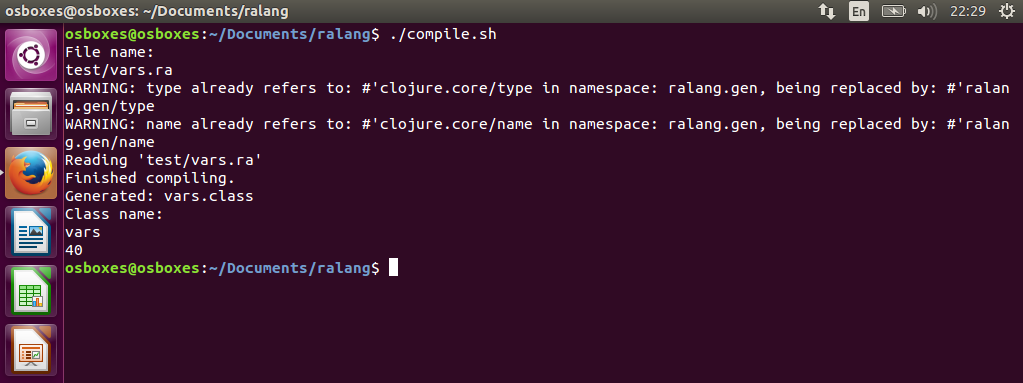
\includegraphics[width=\linewidth]{images/ubuntu_vars.png}
		\caption[Compiling and running vars.ra on Ubuntu 15.10 64-bit]{Compiling and running vars.ra on Ubuntu}
		\label{fig:ubuntu_vars}
	\end{figure}
	\begin{figure}[h!]
		\centering
		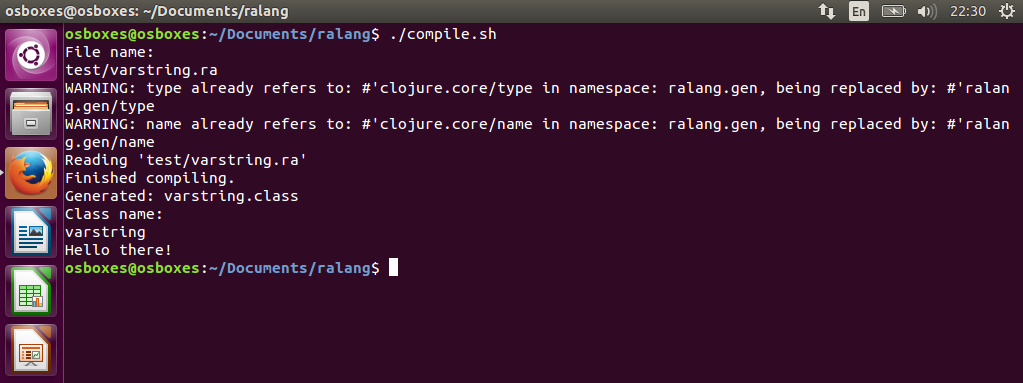
\includegraphics[width=\linewidth]{images/ubuntu_varstring.png}
		\caption[Compiling and running varstring.ra on Ubuntu 15.10 64-bit]{Compiling and running varstring.ra on Ubuntu}
		\label{fig:ubuntu_varstring}
	\end{figure}
	\newpage
	\subsection{Windows - Windows 10 32-bit}
	\begin{figure}[h!]
		\centering
		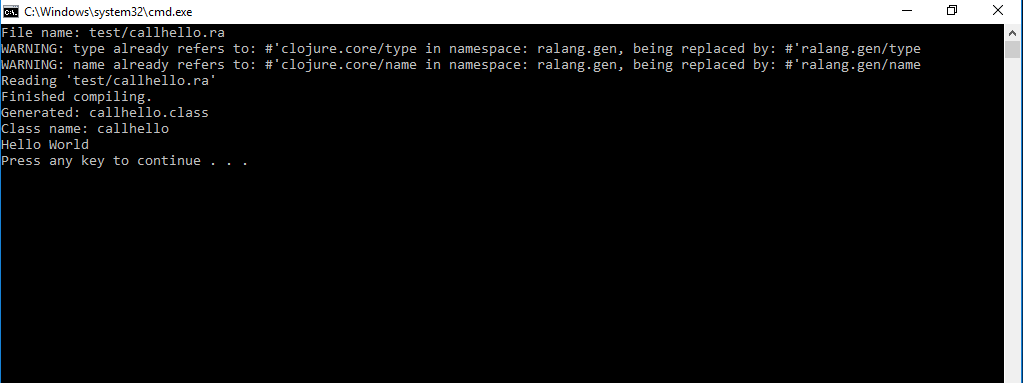
\includegraphics[width=\linewidth]{images/windows_callhello.png}
		\caption[Compiling and running callhello.ra on Windows 10 32-bit]{Compiling and running callhello.ra on Windows}
		\label{fig:windows_callhello}
	\end{figure}
	\begin{figure}[h!]
		\centering
		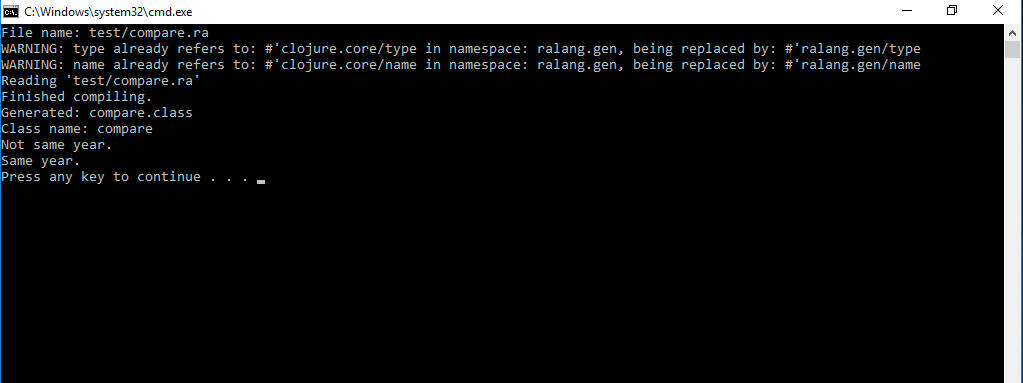
\includegraphics[width=\linewidth]{images/windows_compare.png}
		\caption[Compiling and running compare.ra on Windows 10 32-bit]{Compiling and running compare.ra on Windows}
		\label{fig:windows_compare}
	\end{figure}
	\begin{figure}[h!]
		\centering
		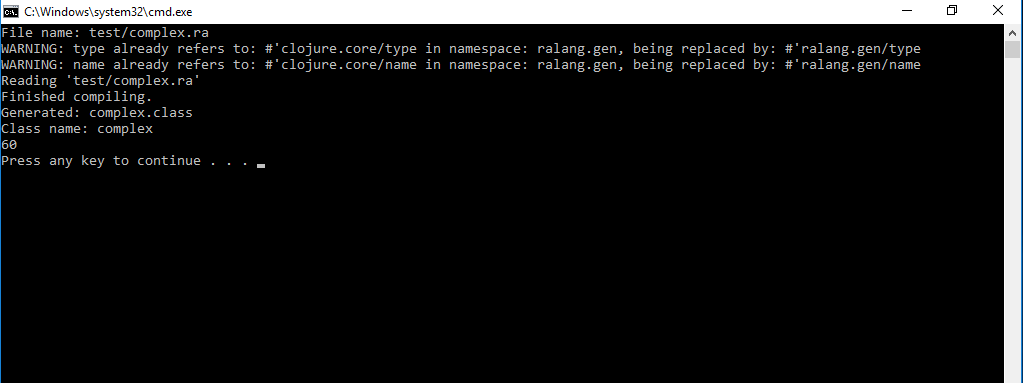
\includegraphics[width=\linewidth]{images/windows_complex.png}
		\caption[Compiling and running complex.ra on Windows 10 32-bit]{Compiling and running complex.ra on Windows}
		\label{fig:windows_complex}
	\end{figure}
	\newpage
	\begin{figure}[h!]
		\centering
		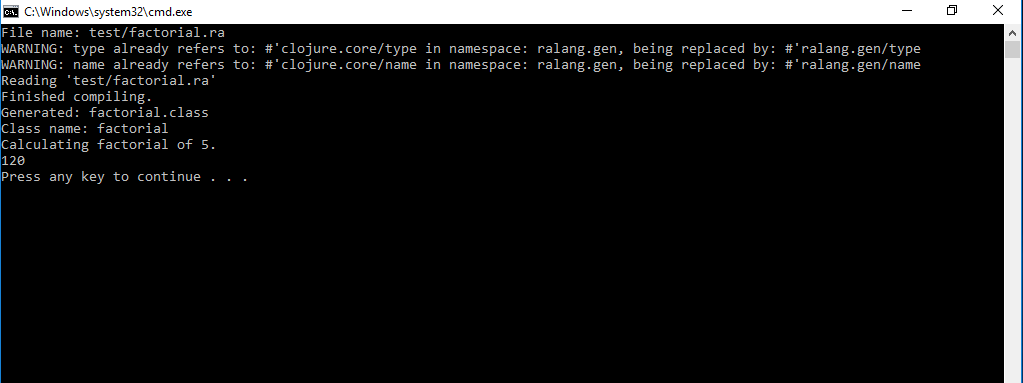
\includegraphics[width=\linewidth]{images/windows_factorial.png}
		\caption[Compiling and running factorial.ra on Windows 10 32-bit]{Compiling and running factorial.ra on Windows}
		\label{fig:windows_factorial}
	\end{figure}
	\begin{figure}[h!]
		\centering
		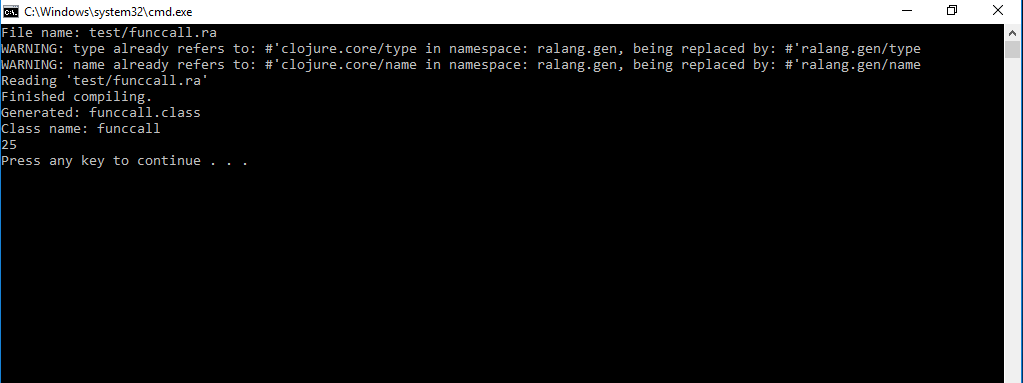
\includegraphics[width=\linewidth]{images/windows_funccall.png}
		\caption[Compiling and running funccall.ra on Windows 10 32-bit]{Compiling and running funccall.ra on Windows}
		\label{fig:windows_funccall}
	\end{figure}
	\begin{figure}[h!]
		\centering
		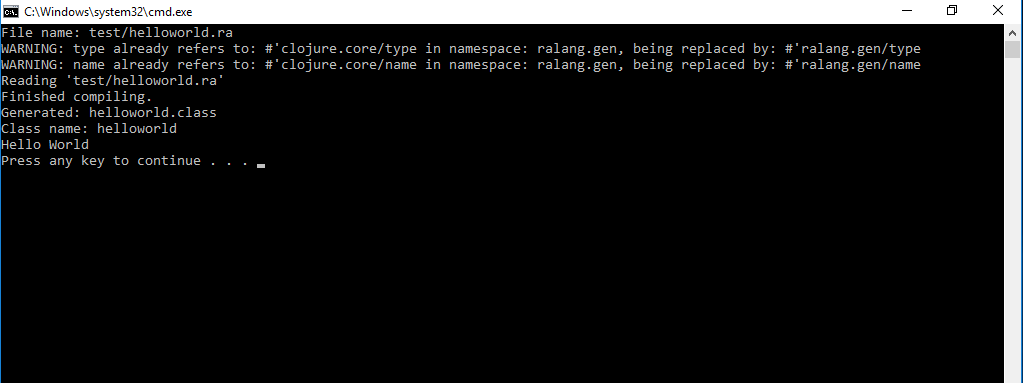
\includegraphics[width=\linewidth]{images/windows_helloworld.png}
		\caption[Compiling and running helloworld.ra on Windows 10 32-bit]{Compiling and running helloworld.ra on Windows}
		\label{fig:windows_helloworld}
	\end{figure}
	\newpage
	\begin{figure}[h!]
		\centering
		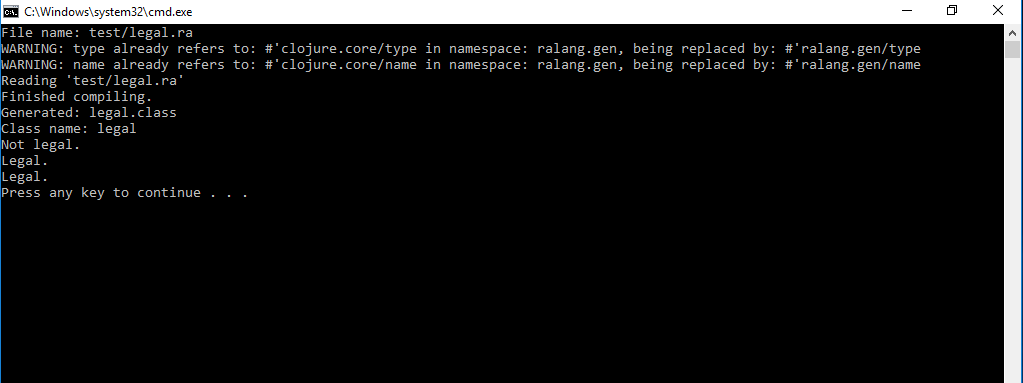
\includegraphics[width=\linewidth]{images/windows_legal.png}
		\caption[Compiling and running legal.ra on Windows 10 32-bit]{Compiling and running legal.ra on Windows}
		\label{fig:windows_legal}
	\end{figure}
	\begin{figure}[h!]
		\centering
		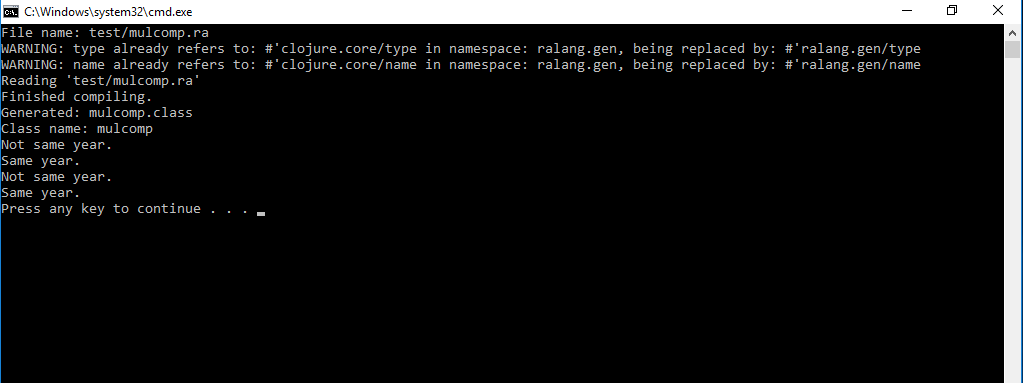
\includegraphics[width=\linewidth]{images/windows_mulcomp.png}
		\caption[Compiling and running mulcomp.ra on Windows 10 32-bit]{Compiling and running mulcomp.ra on Windows}
		\label{fig:windows_mulcomp}
	\end{figure}
	\begin{figure}[h!]
		\centering
		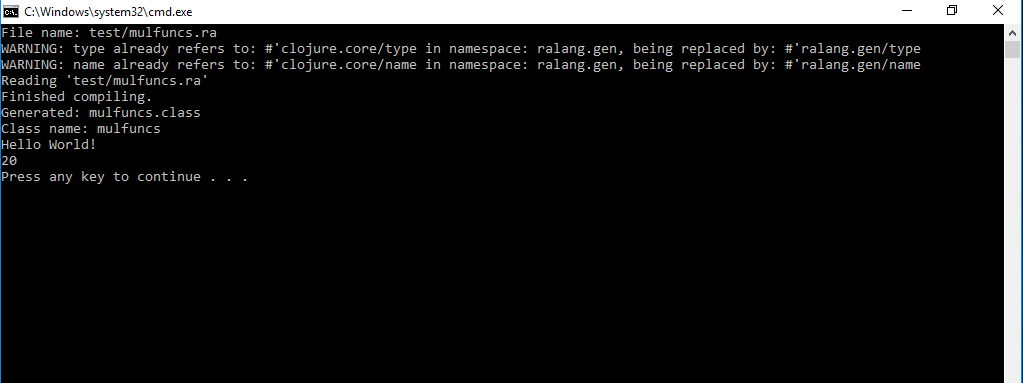
\includegraphics[width=\linewidth]{images/windows_mulfuncs.png}
		\caption[Compiling and running mulfuncs.ra on Windows 10 32-bit]{Compiling and running mulfuncs.ra on Windows}
		\label{fig:windows_mulfuncs}
	\end{figure}
	\newpage
	\begin{figure}[h!]
		\centering
		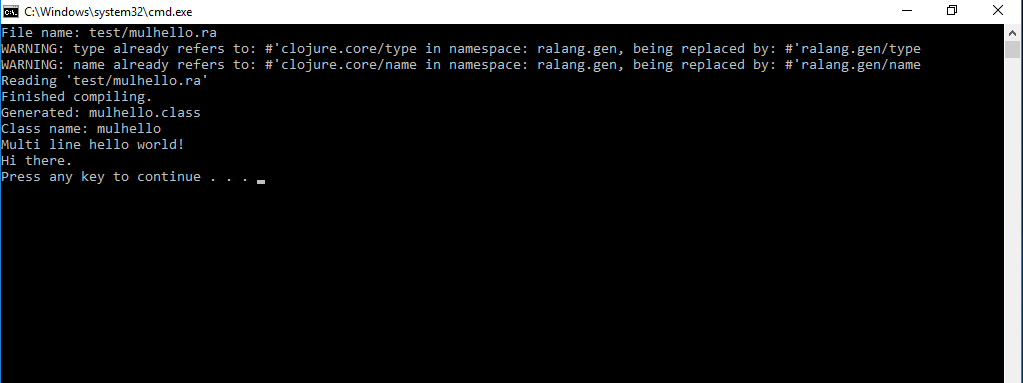
\includegraphics[width=\linewidth]{images/windows_mulhello.png}
		\caption[Compiling and running mulhello.ra on Windows 10 32-bit]{Compiling and running mulhello.ra on Windows}
		\label{fig:windows_mulhello}
	\end{figure}
	\begin{figure}[h!]
		\centering
		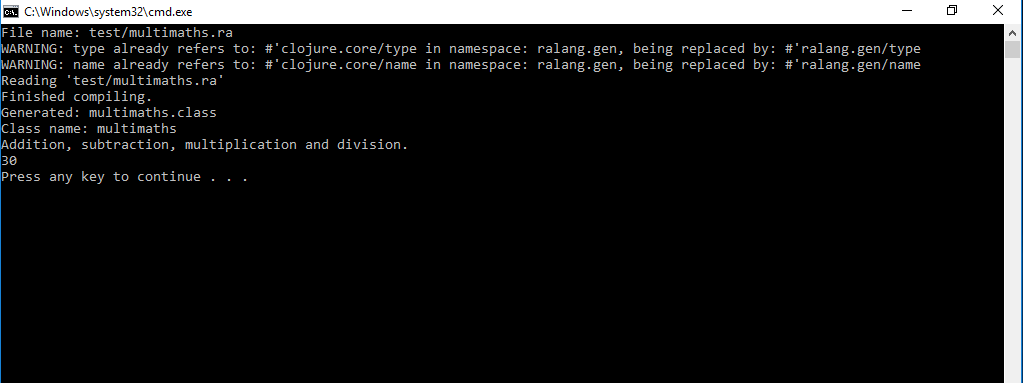
\includegraphics[width=\linewidth]{images/windows_multimaths.png}
		\caption[Compiling and running multimaths.ra on Windows 10 32-bit]{Compiling and running multimaths.ra on Windows}
		\label{fig:windows_multimaths}
	\end{figure}
	\begin{figure}[h!]
		\centering
		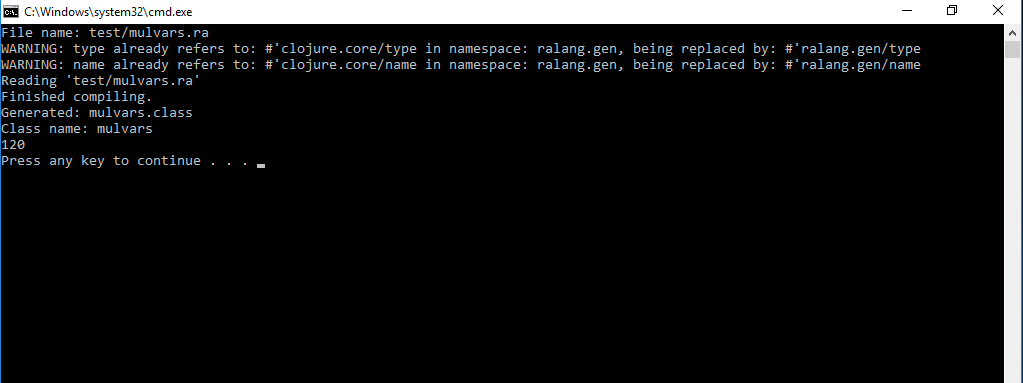
\includegraphics[width=\linewidth]{images/windows_mulvars.png}
		\caption[Compiling and running mulvars.ra on Windows 10 32-bit]{Compiling and running mulvars.ra on Windows}
		\label{fig:windows_mulvars}
	\end{figure}
	\newpage
	\begin{figure}[h!]
		\centering
		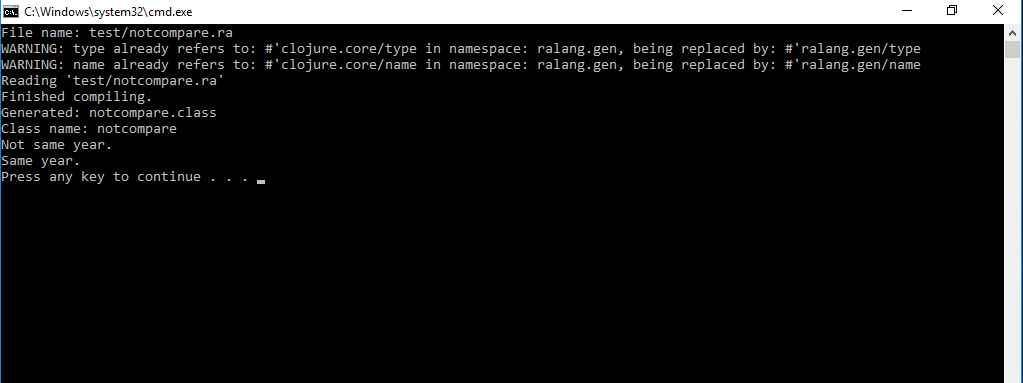
\includegraphics[width=\linewidth]{images/windows_notcompare.png}
		\caption[Compiling and running notcompare.ra on Windows 10 32-bit]{Compiling and running notcompare.ra on Windows}
		\label{fig:windows_notcompare}
	\end{figure}
	\begin{figure}[h!]
		\centering
		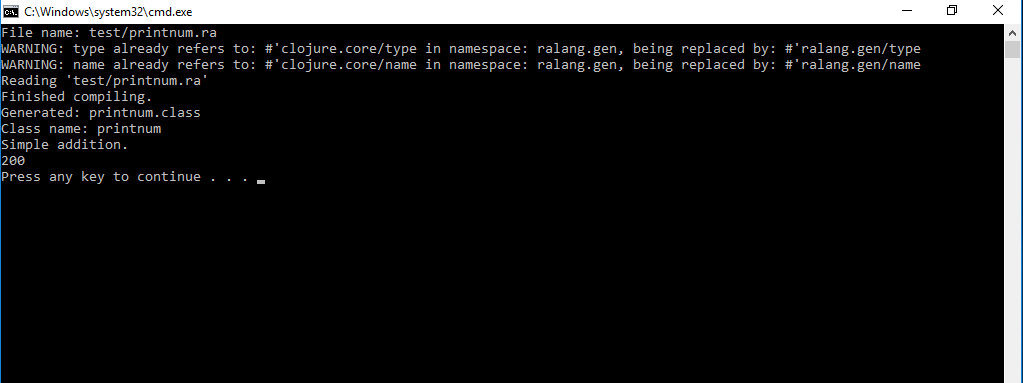
\includegraphics[width=\linewidth]{images/windows_printnum.png}
		\caption[Compiling and running printnum.ra on Windows 10 32-bit]{Compiling and running printnum.ra on Windows}
		\label{fig:windows_printnum}
	\end{figure}
	\begin{figure}[h!]
		\centering
		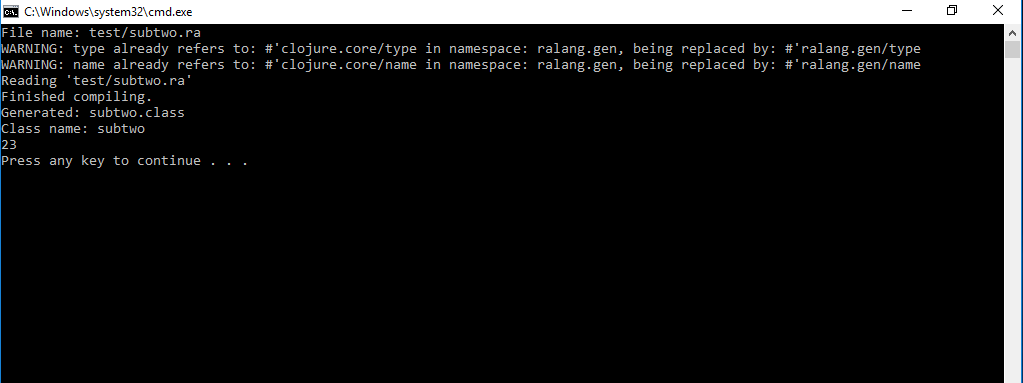
\includegraphics[width=\linewidth]{images/windows_subtwo.png}
		\caption[Compiling and running subtwo.ra on Windows 10 32-bit]{Compiling and running subtwo.ra on Windows}
		\label{fig:windows_subtwo}
	\end{figure}
	\newpage
	\begin{figure}[h!]
		\centering
		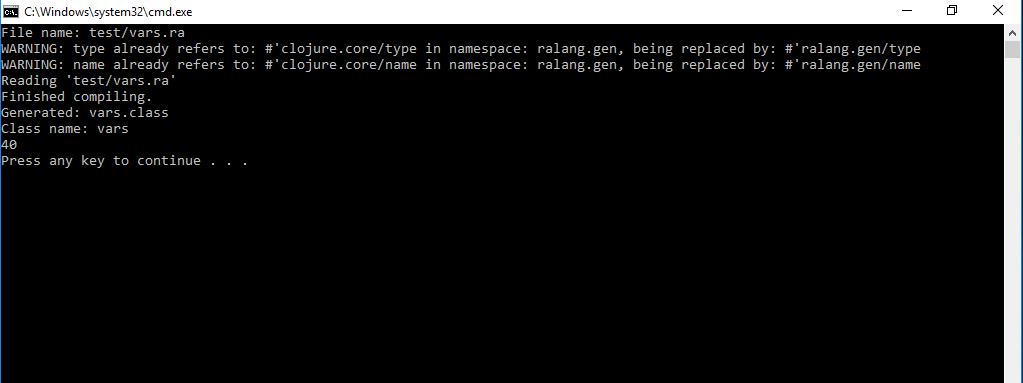
\includegraphics[width=\linewidth]{images/windows_vars.png}
		\caption[Compiling and running vars.ra on Windows 10 32-bit]{Compiling and running vars.ra on Windows}
		\label{fig:windows_vars}
	\end{figure}
	\begin{figure}[h!]
		\centering
		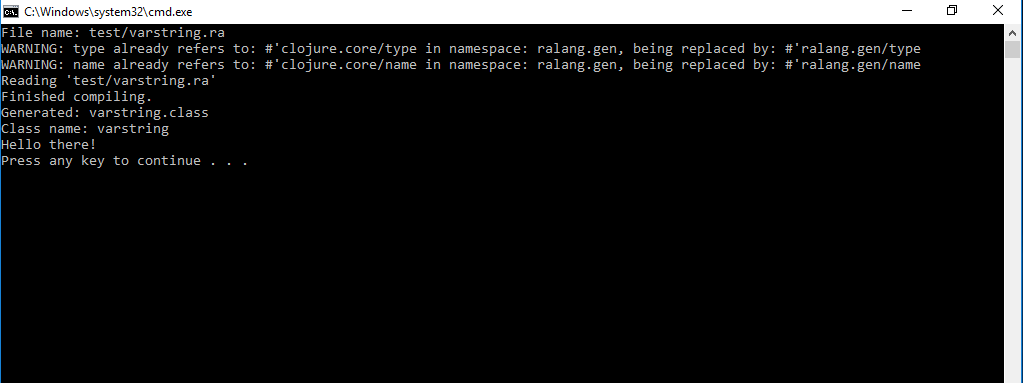
\includegraphics[width=\linewidth]{images/windows_varstring.png}
		\caption[Compiling and running varstring.ra on Windows 10 32-bit]{Compiling and running varstring.ra on Windows}
		\label{fig:windows_varstring}
	\end{figure}
	\newpage
	\section{Java integration}
	\label{App:JavaIntegration}
	\begin{figure}[h!]
		\centering
		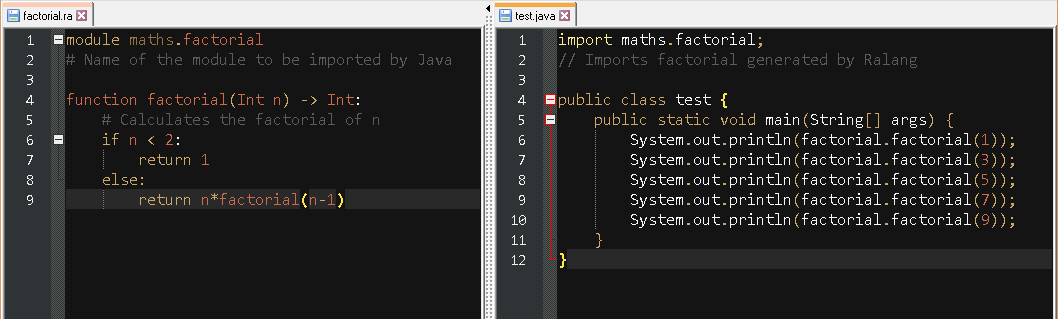
\includegraphics[width=\linewidth]{images/java_import_ralang.png}
		\caption{Importing Ralang module into Java application}
		\label{fig:ImportRalang}
	\end{figure}
	\begin{figure}[h!]
		\centering
		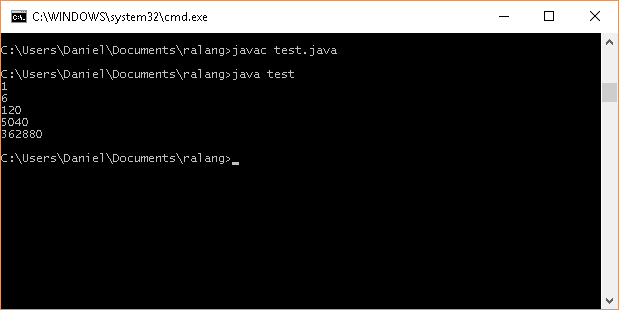
\includegraphics[width=\linewidth]{images/test_java_ralang.png}
		\caption{Running Java application after importing Ralang class}
		\label{fig:RunningJavaApp}
	\end{figure}
	\newpage
	\section{High-level design}
	\label{App:HighLevelDesign}
	\begin{figure}[h!]
		\centering
		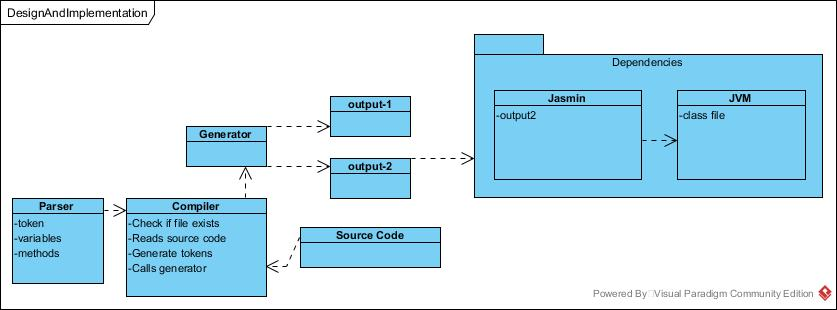
\includegraphics[width=0.95\linewidth]{images/DesignAndImplementation}
		\caption[High level design of Ralang compiler]{High-level design of Ralang compiler}
		\label{fig:DesignAndImplementation}
	\end{figure}
	\pagebreak	
	\section{Proposal - Introduction}
	\label{App:ProposalIntro}
	Computer programming is across a range of different subjects such as Computer Science, Biology, Mathematics, Physics, etc. For that reason the first programming language is very important and critical choice to make. When the programming language is too hard students will become overwhelmed with the amount of work they have to do and might give up on the subject whilst if it's too easy then the students will be under qualified for a job after they graduate.
	
	\subsection{Aim}
	The aim of this project is to design and implement a compiler for a programming language to assist students currently enrolled in a computer science degree. This language is purely education and is not meant to replace any existing language currently in use, but to compliment them by providing the same functionality in a neater syntax so that students can familiarise themselves with computer programming instead of running into problems caused by syntactically incorrect programs as described by \textcite{KrpanBilobrk2011}.
	
	\subsection{Objectives}
	\begin{enumerate}
		\item The syntax of the language should be relatively easy for students taking a programming module in higher education. This can be evaluated by carrying out a simple test along with a questionnaire. Using statistics to compare the results to previous tests, the outcome of the tests can be obtained relatively quick as soon as the questionnaires have been filled in and the tests completed.
		\item Given the amount of time provided to complete this project it's important to only focus on improving the correctness of the program rather the program's efficiency. \textcite{AhoLamSethiUllman2006} says the code optimisation process must also be correct to preserve the meaning of the compiled program, this means focusing more on the code generation will achieve better results overall. It will then be possible to execute pre-defined test programs and data to evaluate whether the compiler provides the correct results.
		\item The compiler is able to compile source code both for Linux and Windows operating system. Various number of tests will be used to check if the program performance has a significant changes in both these Operating Systems, or if they perform at the same level. To do this, a virtual machine will be created and given the same amount of memory, then tests can be performed. Setting up virtual machines and writing the test cases may take some time, nevertheless this will allow the creation of statistics on the data obtained from the results to compare the performance of the programming language in different operating systems.
	\end{enumerate}
	
	\subsection{Research methodologies}
	Only peer-reviewed journals and papers, and books on the compiler writing are going to be used through-out this research. Peer-reviewed journals and papers will be filtered out by skimming through abstracts and introductions, as time is a constraint for this project. The most relevant 10 to 15 journals and papers will be selected for the literature review. Well known books will be referenced in the reference section at the end. Books will only be used if there are no relevant papers on the subject.
	
	\newpage
	\section{Proposal - Literature review}
	\label{App:LitReview}
	\subsection{Introduction}
	Computer programming is a fundamental requirement at any Bachelor of Science degree such as physics, biology and computer science. Nevertheless, learning a programming language can be a difficult and taunting challenge for people who have not programmed before. \textcite{VihavainenAiraksinenWatson2014} says despite the enormous efforts to improve CS failure rates, these numbers are still very high across the board. Institutions also have to ensure students enrolled in computer programming courses are able to understand the content of the course and at the same time the students must be prepared to use the skills gained to go into industry confident and able to perform the required jobs. \parencite{KrpanBilobrk2011}\\
	
	This literature review attempts to answer two main questions: What do the majority students enrolled on a computer programming course find difficult and how can this problem be tackled. How the problem can be tackled also needs to take into consideration programming languages currently being used in the industry, and whether learning a certain pedagogical language, would enable the students to transit to another industry programming language such as Java, C\# or C++ for example.
	
	\subsection{Introductory programming languages}
	There are various different approaches to the problem of what programming languages are better to learn as a introductory language. \textcite{Daly2011} compares using Alice/Java course against a pure Java course. Alice is a object-oriented 3D programming environment used to introduce students to computer programming. The results carried out of this research found that students learning Java along with Alice were a lot more confident than those learning pure Java. Even though \textcite{Daly2011} concludes that students that learn Alice alongside Java seem to be more enthusiastic about taking another programming course than those that learn pure Java, it failed to address the issue of how well the students actually performed in the end in terms of being able to write a simple computer program.\\
	
	\textcite{KrpanBilobrk2011} takes a similar approach to the problem above but this time around students are learning C, QBasic and Python. In this experiment the students attempt 3 different exercises: calculating factorial of n, reversing a string and counting words in a text file. The students seemed more confident about programming in Python, and rated C as the most difficult programming language to use, nevertheless achieved an overall better results in the C language.\\
	
	\begin{wrapfigure}{l}{0.5\textwidth}
		\vspace{-20pt}
		\begin{center}
			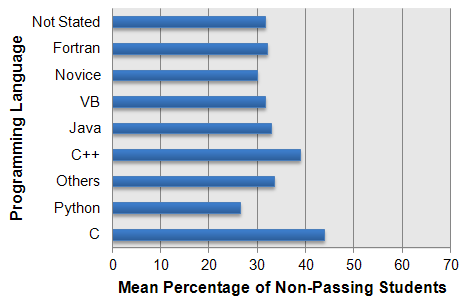
\includegraphics[width=0.48\textwidth]{NonPassingStudents}
		\end{center}
		\caption[Non-passing students grouped by programming language]{Non-passing students grouped by programming language. \parencite{WatsonLi2014}}
		\vspace{-10pt}
	\end{wrapfigure}
	
	\textcite{WatsonLi2014} obtained a more comprehensive set of results by combining data from 145 universities and 16 college from various different countries and looking at the top programming languages used at these institutions. Figure 1, compares Fortran, Novice, VB, Java, C++, Python, C and other languages. Python programming language in this case achieves the best mean percentage, whilst C programming language seems to get more non-passing students, nevertheless as mentioned in \textcite{WatsonLi2014}, the mean percentage of non-passing students does not seem to vary extraordinarily as the results range from 25\% to 45\% and remains consistent throughout.\\
	
	In \textcite{WatsonLi2014}, shows that there are trends mean percentage of non-passing students is actually decreasing over the years. This could be due to the fact that easier to learn programming languages are being introduced, and therefore it is easier for students to pass. This does not necessarily mean that students will be able to solve problems by themselves after they finish the computer programming course, and this could be an issue in the future.\\
	
	Another problem is whether the students will be able to tackle issues by themselves when they finish their course. \textcite{JayalLauriaTuckerSwift2011} says that there is a positive increase in the number of students taking Python as their first programming language. It reason that students taking Python can focus more on the problems themselves rather than syntactic issues. This means that students taking Python as their first language are more likely to be able to tackle issues by themselves.\\
	
	Python is getting a lot of popularity in computer programming course as an introductory language. \parencite{Yadin2011} Python programs allow students to focus on the procedural programming allowing them to think of problems and how to solve them using algorithms. Students tend to find object-oriented programming and this could be the reason why Java seems to lower the confidence levels in students when taught as a first programming language like shown in \textcite{Daly2011}. In fact, many institutions were able to lower the drop out rate by introduction Python as an introductory programming language. \parencite{NikulaSajaniemiTedreWray2007}\\
	
	Similar issues apply when teaching functional programming to first years. \textcite{ChakravartyKeller2004} says that functional programming is hardly a good idea for a student who has never came across programming before. 
	
	\subsection{Conclusion}
	At various different institutions around the world different approaches are being taken to lower the number of drop out and to increase the number of students who will be motivated enough to pursue another computer programming course. A lot of these institution seem to be preferring a Python approach to this problem, and drop outs seem to be decreasing. \parencite{JayalLauriaTuckerSwift2011}\\
	
	Nevertheless, the trend doesn't seem to be mutual across every institution as the results tends to vary and indicate otherwise as observed by \textcite{KrpanBilobrk2011} where the average students preferred Python but achieved an overall better grade in C. A slight different case where students across 144 different universities obtained about the same performance in different languages, suggesting the language might not impact how well students solve problems using the computer. \parencite{WatsonLi2014}\\
	
	It's also important to note that students learning procedural programming rather than objected-oriented or functional programming, are able to perform better when it comes to writing algorithms and solving problems. \parencite{Kolling1999}\\
	
	It is also important to note that most of the statistics provided in the above papers were very limited and might not represent fully correct data, as only samples were collected. The largest sample of data found was done to 161 institutions from all around the world.
	\newpage
	\section{Proposal - Design}
	\label{App:ProposalDesign}
	\subsection{Requirement specification}
	\label{App:RequirementSpecification}
	Ralang source code should be easy to read and easy to write. By comparing Java source code with Ralang source code in Figure 2. it's clear that Ralang requires less lines of code and less characters to print "Hello, World" to the screen, meaning that student will have to write much less to obtain the same results.\\
	
	Objective 3 for this project is that the compiler for Ralang must be able to run both on Windows and Linux operating system. In order to make that happen the source code of the program is compiled to Java bytecode to run on the Java Virtual Machine. There are several languages that will run on the \ac{jvm} such as Java, Scala, Clojure and Jython. A functional programming would be more suitable for this project because of compiler work a lot with trees and also pattern matching, in which case Clojure may be very suitable.\\
	
	To understand whether the programming language meets the requirements, a simple test along with a questionnaire will be carried out to first and second year students, who may have prior programming knowledge and they will be required to follow a written or video tutorial, then write a simple application and finally answer some questionnaire questions about how they feel about the language.\\
	
	\textcite{AhoLamSethiUllman2006} lays out the seven different phases to writing a compiler: Lexical, syntax and semantic analyser, intermediate code generator, machine-independent code optimiser, code generator and machine-dependent code optimizer. To ensure the project can be successfully completed within a certain time frame, code optimisation will be skipped. In that case more time can be spent to ensure the correctness of the compiler.\\
	
	From the literature review, it was concluded that the Python programming language is used to at various institutions to introduce students to computer programming, nevertheless many students claimed Python was far easier than languages like C but still the overall average performed better in C. \parencite{KrpanBilobrk2011}\\
	
	It was understood the majority of people preferred Python because of its neat and clear syntax but due to being a dynamic programming language students tend to have many problem being able to write and run their own programs.  Ralang will implement static typing, where the compiler will do various checks and report errors where possible but also implement a neat and clear syntax like Python.
	
	\subsection{Development methodologies}
	\label{App:DevelopmentMethodology}
	There are several development methodologies available to use for this project such as \ac{rad} or scrum software development.\\
	
	Scrum software development assumes that the problem can not be completely laid out, and changes may be made along the way. This methodology allows quick prototyping and would allow quick deliverables, so it would work well for projects that would require to be changed frequently.\\
	
	Similarly, \ac{rad} provides a fast development process and it's easy to adjust to the requirements of the project. It will allow easy prototyping and making changes as necessary to obtain best results possible, whether that would be the correctness of the program, or changes to the syntax of language or even how to deal with compiling errors.\\
	
	\ac{rad} seems the most suitable methodology as the development of the project won't be altering constantly, there might be slight changes along the way until the final product is complete, nevertheless the changes will always be minor until the end product is finished.
	\newpage
	\section{Research Questionnaire}
	\label{App:Questionnaire}
	\begin{figure}[h!]
		\centering{
		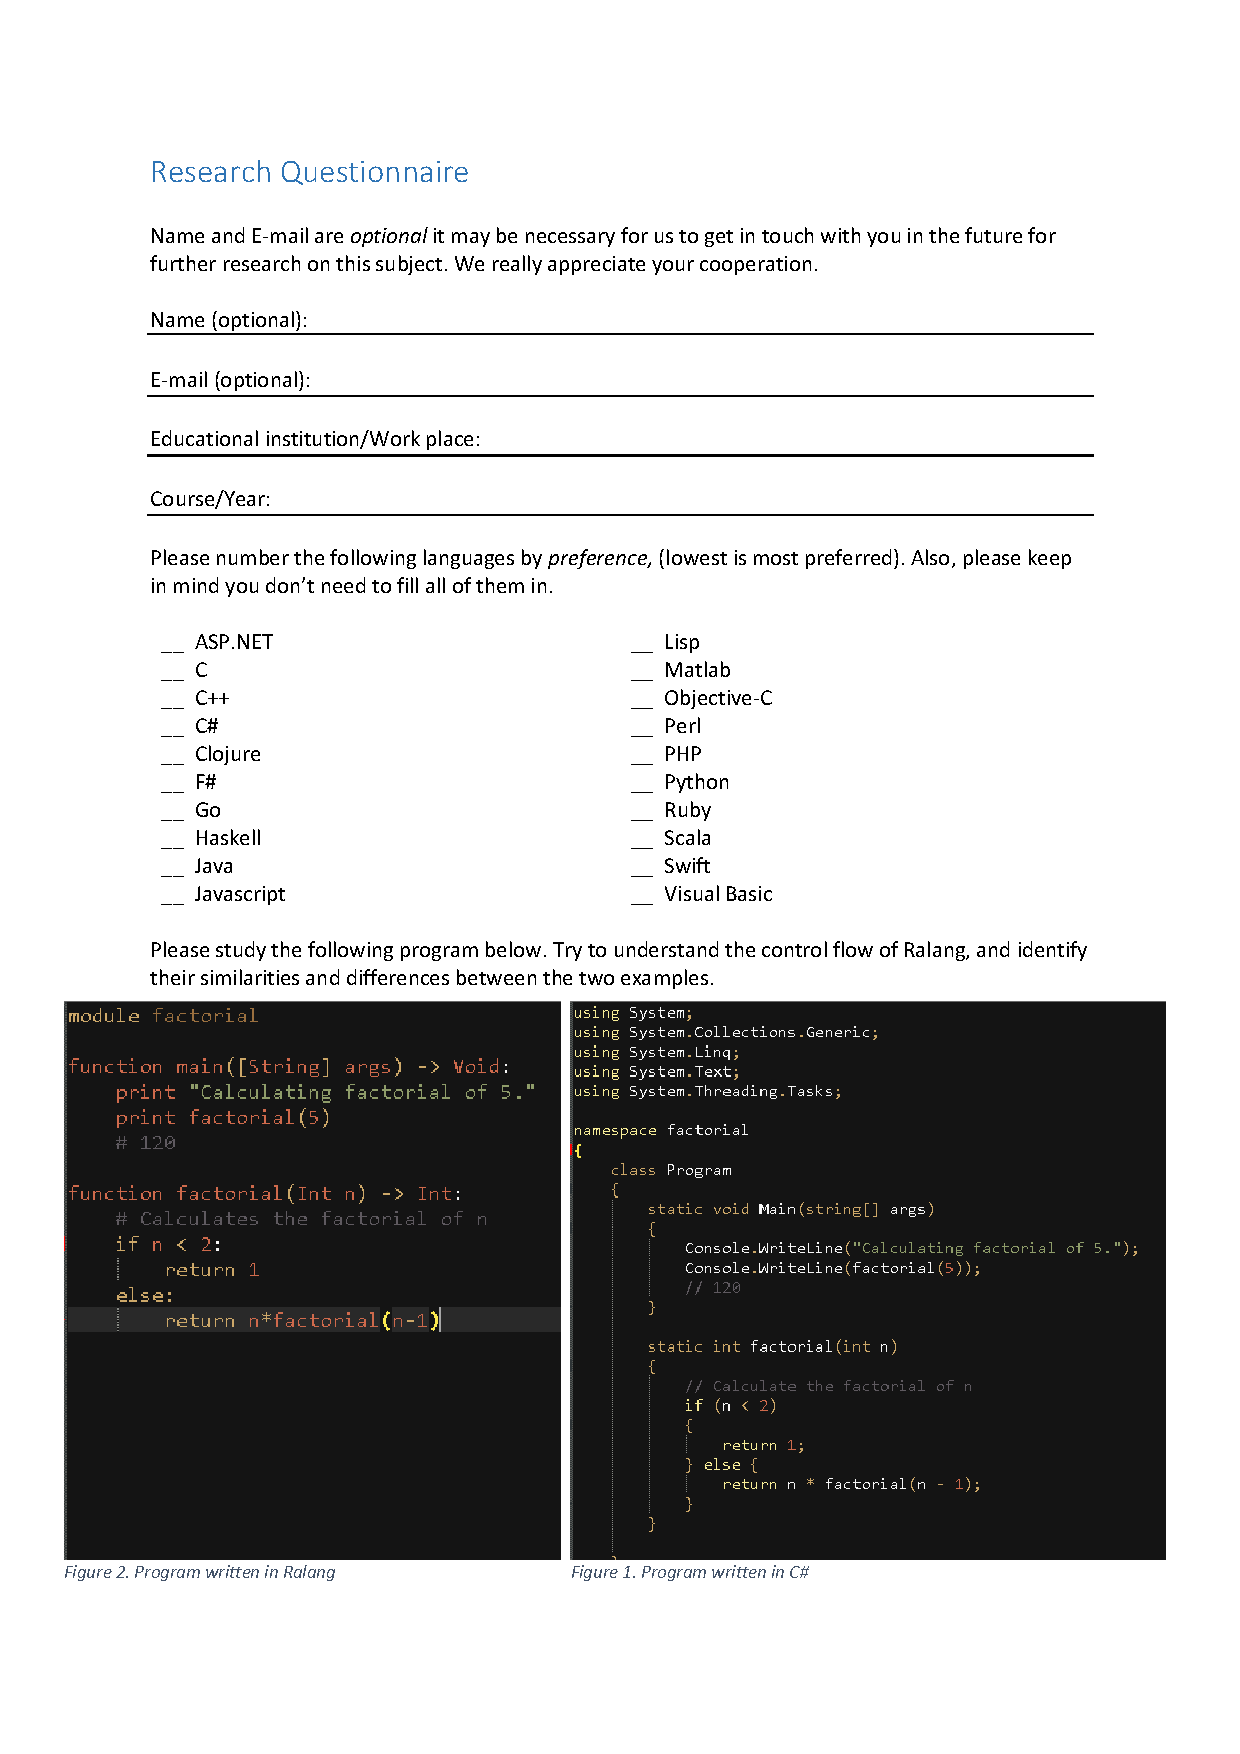
\includegraphics[width=\linewidth]{ResearchQuestionnaire1.pdf}}
		\caption{Research Questionnaire about Ralang's syntax - Page 1}
	\end{figure}
	\newpage
	\begin{figure}[h!]
		\centering{
			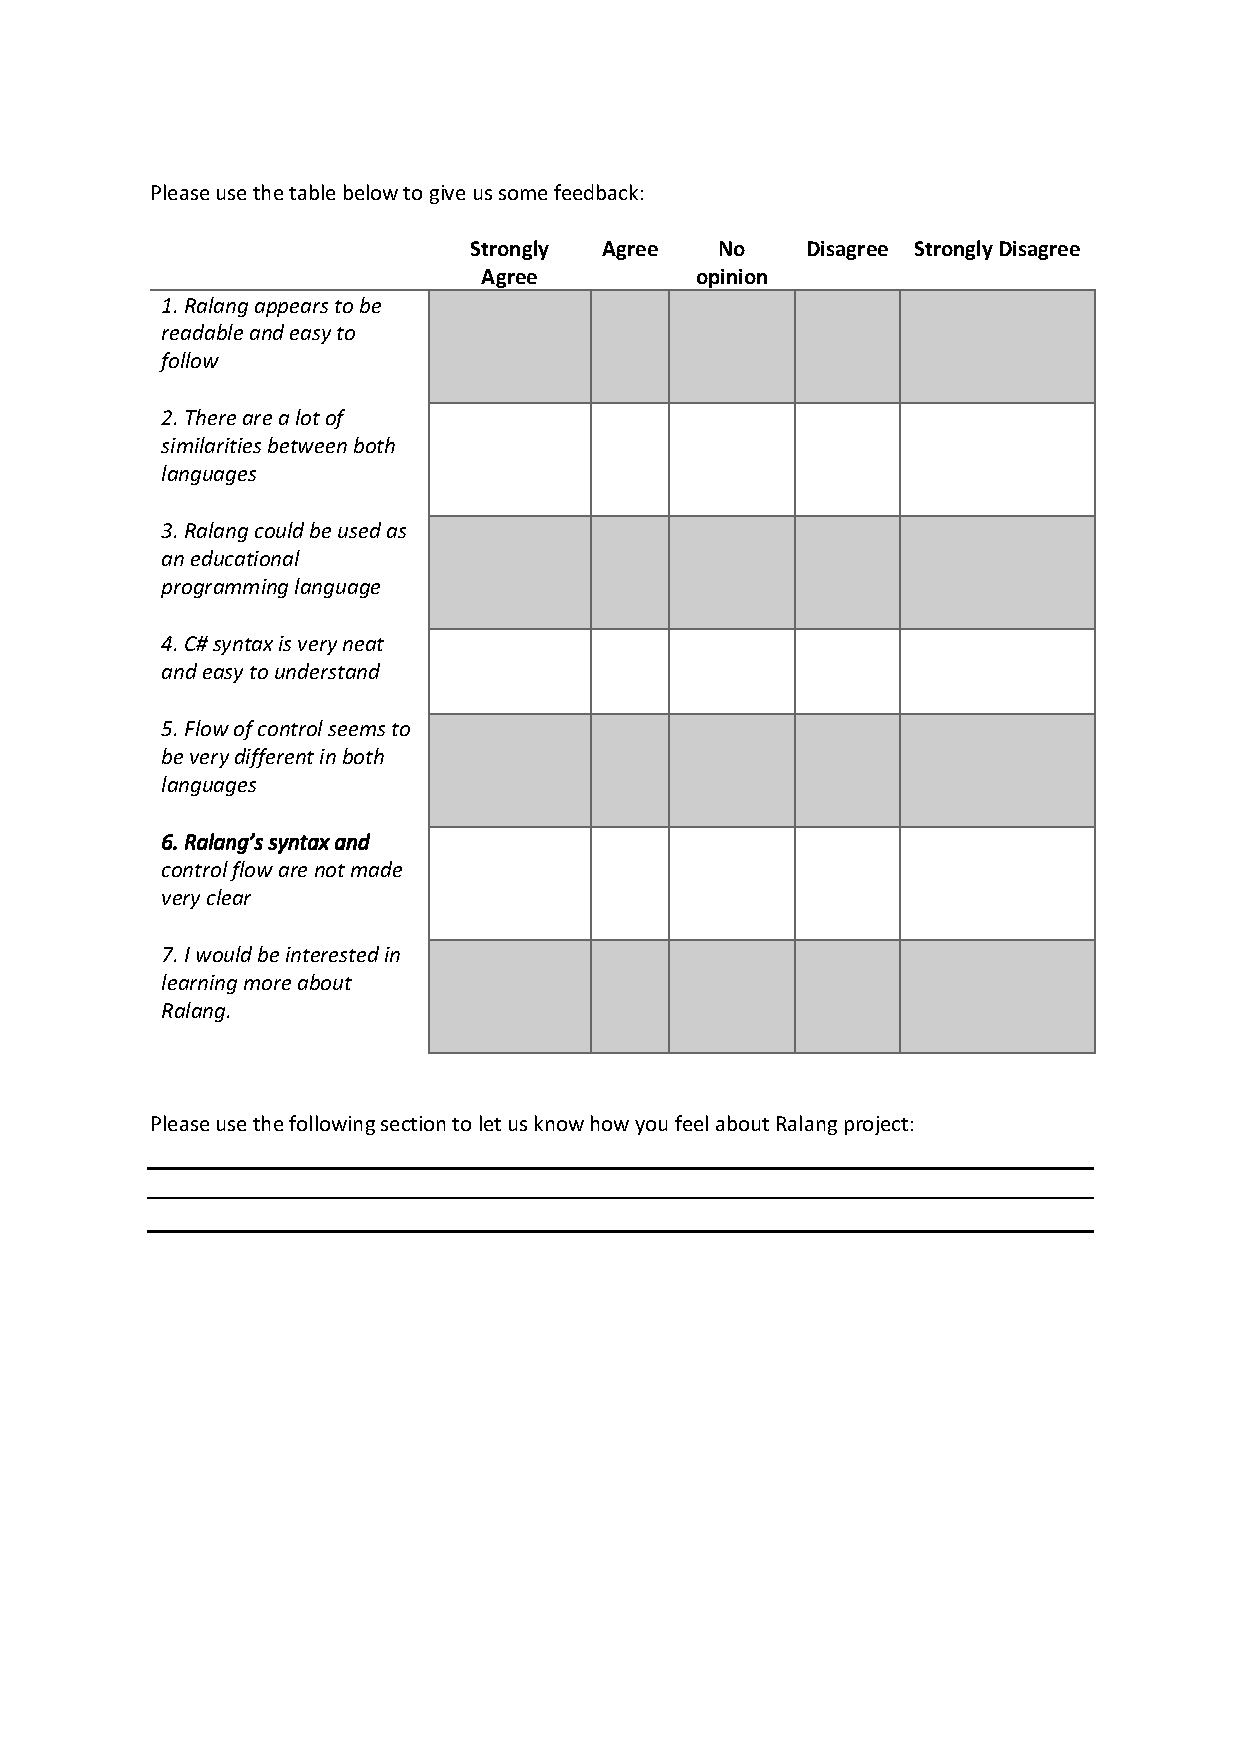
\includegraphics[width=\linewidth]{ResearchQuestionnaire2.pdf}}
		\caption{Research Questionnaire about Ralang's syntax - Page 2}
	\end{figure}
	\newpage
	\section{Questionnaires}
	\begin{figure}[h!]
		\centering{
			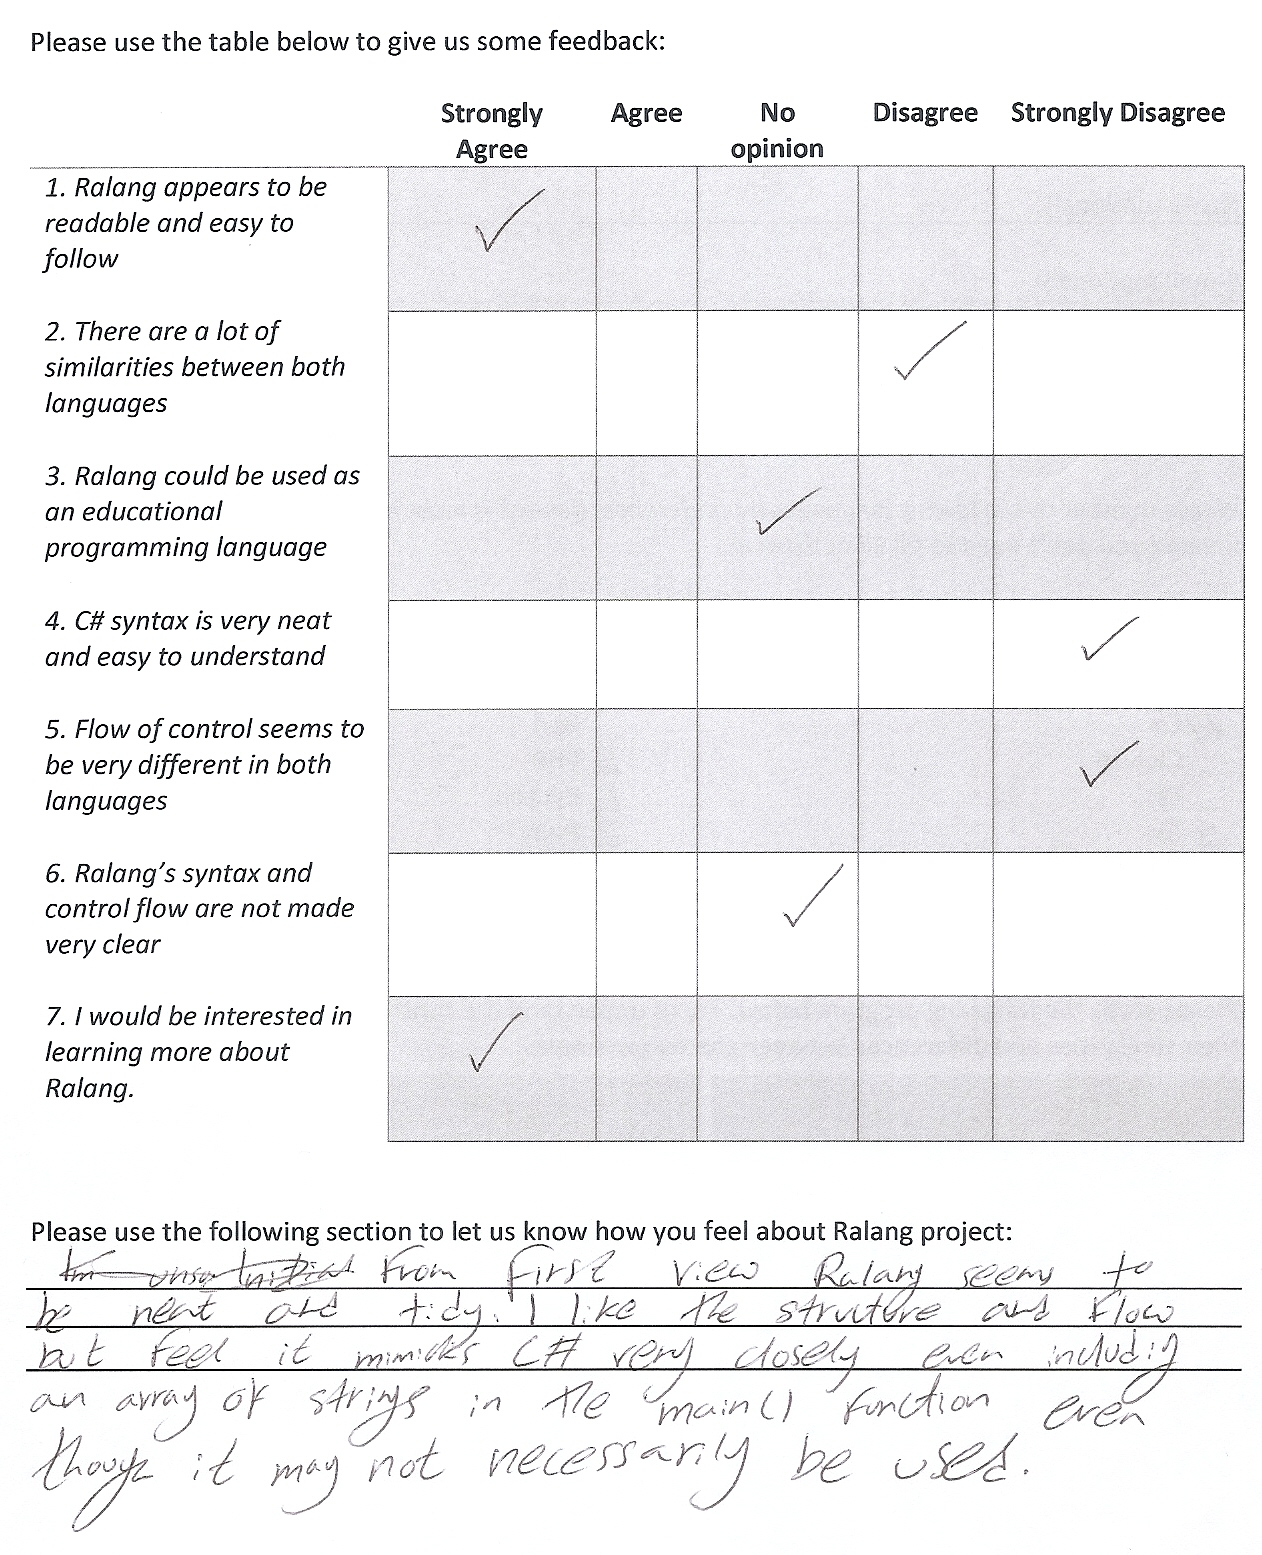
\includegraphics[width=\linewidth]{images/scan1.jpg}}
		\caption{Research Questionnaire - Answer sheet number 1}
	\end{figure}
	\newpage
	\begin{figure}[h!]
		\centering{
			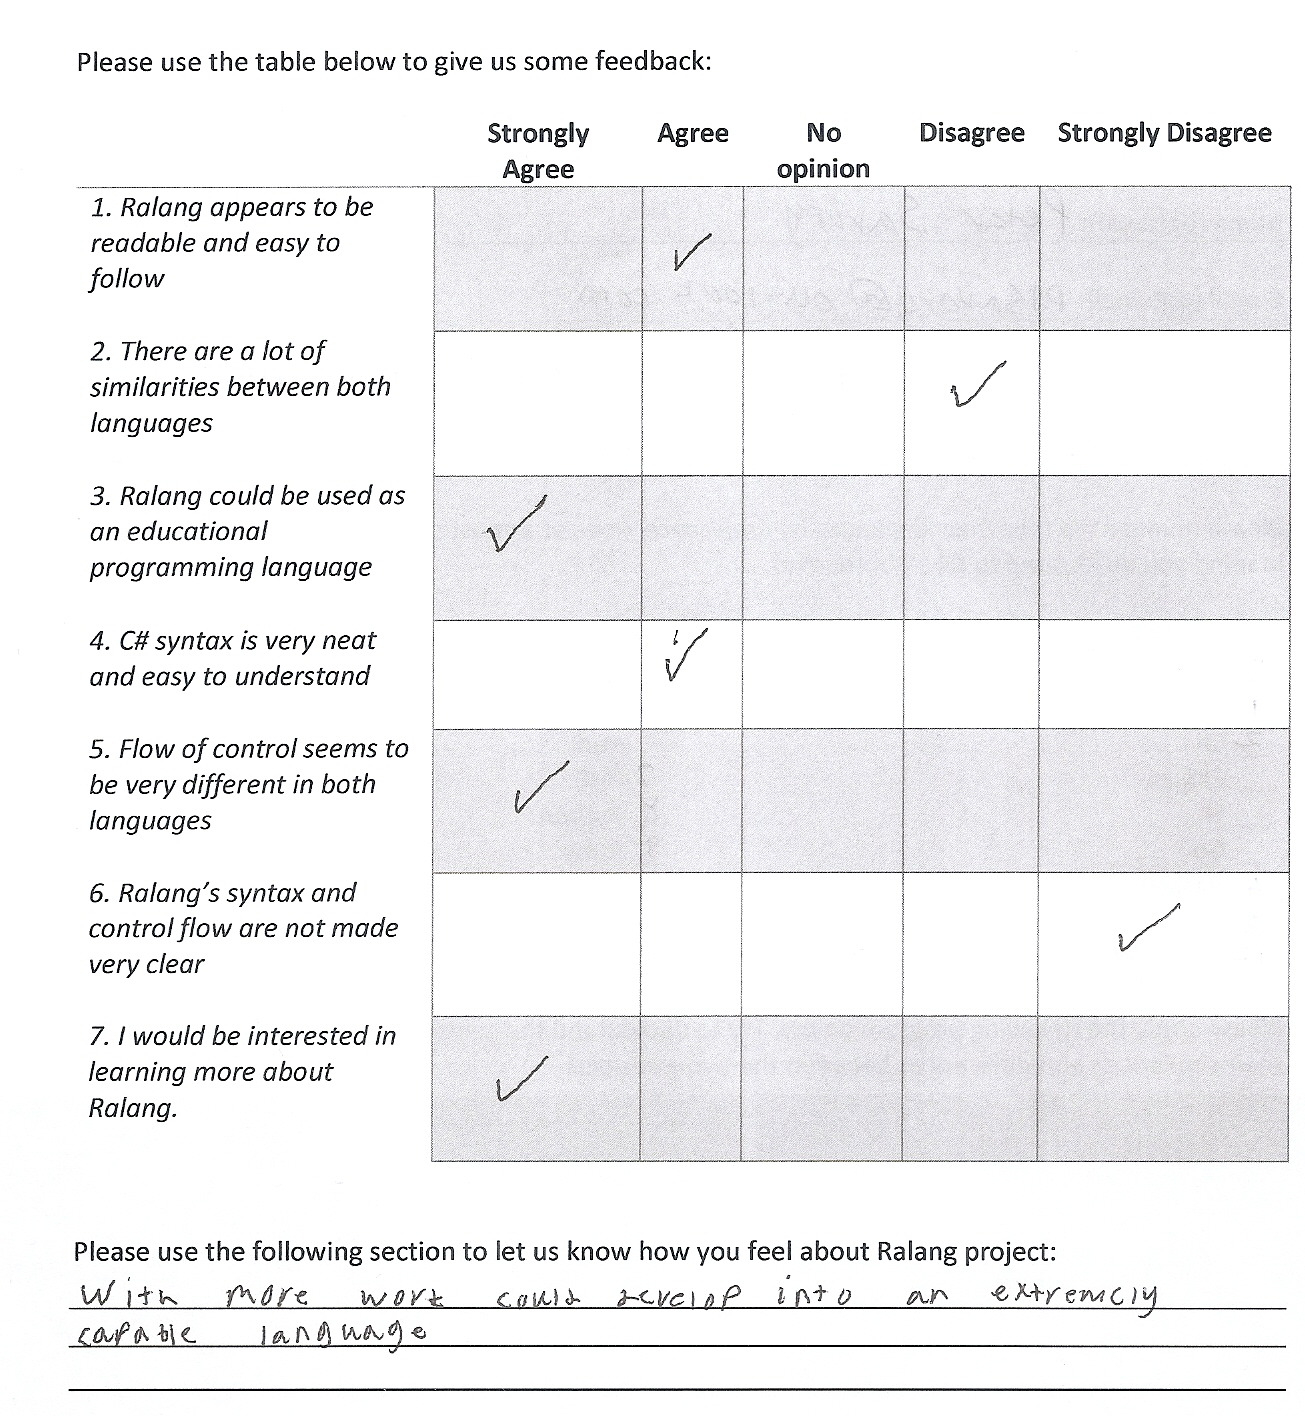
\includegraphics[width=\linewidth]{images/scan2.jpg}}
		\caption{Research Questionnaire - Answer sheet number 2}
	\end{figure}
	\newpage
	\begin{figure}[h!]
		\centering{
			\includegraphics[width=\linewidth]{images/scan3.jpg}}
		\caption{Research Questionnaire - Answer sheet number 3}
	\end{figure}
	\newpage
	\begin{figure}[h!]
		\centering{
			\includegraphics[width=\linewidth]{images/scan4.jpg}}
		\caption{Research Questionnaire - Answer sheet number 4}
	\end{figure}
	\newpage
	\begin{figure}[h!]
		\centering{
			\includegraphics[width=\linewidth]{images/scan5.jpg}}
		\caption{Research Questionnaire - Answer sheet number 5}
	\end{figure}
	\newpage
	\begin{figure}[h!]
		\centering{
			\includegraphics[width=\linewidth]{images/scan6.jpg}}
		\caption{Research Questionnaire - Answer sheet number 6}
	\end{figure}
	\newpage
	\begin{figure}[h!]
		\centering{
			\includegraphics[width=\linewidth]{images/scan7.jpg}}
		\caption{Research Questionnaire - Answer sheet number 7}
	\end{figure}
	\newpage
	\begin{figure}[h!]
		\centering{
			\includegraphics[width=\linewidth]{images/scan8.jpg}}
		\caption{Research Questionnaire - Answer sheet number 8}
	\end{figure}
	\newpage
	\begin{figure}[h!]
		\centering{
			\includegraphics[width=\linewidth]{images/scan9.jpg}}
		\caption{Research Questionnaire - Answer sheet number 9}
	\end{figure}
	\newpage
	\section{Research Questionnaire - Results}
		Table \ref{Tab:QuestionnaireEvaluation} is used to evaluate the results collected from the research questionnaire. Each of these values will be multiplied by the number of results collected in table \ref{Tab:QuestionnaireResults}.
		\begin{table}[h!]
			\begin{tabular}{|C{3cm}|c|c|c|c|c|}
				\hline  & Strongly Agree & Agree & No opinion & Disagree & Strongly disagree \\ 
				\hline Ralang appears to be readable and easy to follow & 4 & 3 & 2 & 1 & 0 \\ 
				\hline Ralang could be used as an educational programming language & 4 & 3 & 2 & 1 & 0 \\ 
				\hline Ralang's syntax and control flow are not made very clear & 0 & 1 & 2 & 3 & 4 \\ 
				\hline I would be interested in learning more about Ralang & 4 & 3 & 2 & 1 & 0 \\ 
				\hline 
			\end{tabular} \\
			\caption{Contains the values for each cell}
			\label{Tab:QuestionnaireEvaluation}
		\end{table}
		\begin{table}[h!]
			\begin{tabular}{|C{3cm}|c|c|c|c|c|}
			\hline  & Strongly Agree & Agree & No opinion & Disagree & Strongly disagree \\ 
			\hline Ralang appears to be readable and easy to follow & 3 & 5 & 1 & 0 & 0 \\ 
			\hline Ralang could be used as an educational programming language & 3 & 3 & 3 & 0 & 0 \\ 
			\hline Ralang's syntax and control flow are not made very clear & 1 & 1 & 2 & 3 & 2 \\ 
			\hline I would be interested in learning more about Ralang & 5 & 3 & 0 & 1 & 0 \\ 
			\hline 
			\end{tabular} \\
			\caption{Research questionnaire results for N=9}
			\label{Tab:QuestionnaireResults}
		\end{table}
	\newpage
	\section{Presentation}
	\label{App:Presentation}
	\subsection{Slides}
	\begin{figure}[h!]
		\centering{
		\includegraphics[page=1,width=\linewidth]{presentation/RalangPresentationSlides.pdf}}
		\caption{Presentation slides, demonstration and viva slides - Introduction}
	\end{figure}
	\begin{figure}[h!]
		\centering{
			\includegraphics[page=2,width=\linewidth]{presentation/RalangPresentationSlides.pdf}}
		\caption{Presentation slides, demonstration and viva slides - Overview}
	\end{figure}
	\newpage
	\begin{figure}[h!]
		\centering{
		\includegraphics[page=3,width=\linewidth]{presentation/RalangPresentationSlides.pdf}}
		\caption{Presentation slides, demonstration and viva slides - Literature}
	\end{figure}
	\begin{figure}[h!]
		\centering{
			\includegraphics[page=4,width=\linewidth]{presentation/RalangPresentationSlides.pdf}}
		\caption{Presentation slides, demonstration and viva slides - Technologies and tools}
	\end{figure}
	\newpage
	\begin{figure}[h!]
		\centering{
		\includegraphics[page=5,width=\linewidth]{presentation/RalangPresentationSlides.pdf}}
		\caption{Presentation slides, demonstration and viva slides - Design and implementation}
	\end{figure}
	\begin{figure}[h!]
		\centering{
		\includegraphics[page=6,width=\linewidth]{presentation/RalangPresentationSlides.pdf}}
		\caption{Presentation slides, demonstration and viva slides - Tests and questionnaire results}
	\end{figure}
	\newpage
	\begin{figure}[h!]
		\centering{
		\includegraphics[page=7,width=\linewidth]{presentation/RalangPresentationSlides.pdf}}
		\caption{Presentation slides, demonstration and viva slides - Development process}
	\end{figure}
	\begin{figure}[h!]
		\centering{
		\includegraphics[page=8,width=\linewidth]{presentation/RalangPresentationSlides.pdf}}
		\caption{Presentation slides, demonstration and viva slides - Technical issues}
	\end{figure}
	\newpage
	\begin{figure}[h!]
		\centering{
		\includegraphics[page=9,width=\linewidth]{presentation/RalangPresentationSlides.pdf}}
		\caption{Presentation slides, demonstration and viva slides - Further work}
	\end{figure}
	\begin{figure}[h!]
		\centering{
		\includegraphics[page=10,width=\linewidth]{presentation/RalangPresentationSlides.pdf}}
		\caption{Presentation slides, demonstration and viva slides - Resources}
	\end{figure}
	\newpage
	\subsection{Handout}
	\begin{figure}[h!]
		\centering{
			\includegraphics[width=\linewidth]{presentation/Handout.pdf}}
		\caption{Leaflet explaining how to get started with Ralang}
	\end{figure}
	\end{appendices}
\end{document}